\documentclass[a4paper,12pt]{report}
\usepackage[utf8x]{inputenc}
\usepackage{amsmath} % Mathematische Symbole
\usepackage{amssymb} % Mathematische Symbole
\usepackage{graphicx} % Bilder einfügen
\usepackage{subcaption}
\usepackage{verbatim}
\usepackage{mathtools}
\usepackage{subcaption}
\usepackage{wrapfig}
\usepackage[titlenumbered,ruled,linesnumbered]{algorithm2e}
\usepackage{todonotes}
\usepackage{booktabs}
\usepackage[UKenglish]{babel}
\usepackage{float}
\usepackage{epstopdf}
\PassOptionsToPackage{hyphens}{url}\usepackage{hyperref}
\hypersetup{
    citecolor=black,
    filecolor=black,
    linkcolor=green,
    urlcolor=black
}
\usepackage{subcaption}
\usepackage{tabularx}
\usepackage{adjustbox}
\usepackage{textcomp}
\usepackage{flexisym}
\usepackage{listings}
\usepackage{enumerate}
\usepackage{color}
\usepackage[abbreviations,symbols,nogroupskip,nonumberlist]{glossaries-extra}
\usepackage{setspace}
\usepackage{babel,blindtext}
\usepackage[nottoc]{tocbibind}
\usepackage{breakcites}
\usepackage[round]{natbib}
\setcitestyle{square}
%\singlespacing
\makeglossaries[abbreviations]
\newabbreviation{ai}{AI}{Artificial Intelligence}
\newabbreviation{ocr}{OCR}{Optical Character Recognition}
\newabbreviation{gan}{GAN}{Generative Adversarial Network}
\newabbreviation{ssim}{SSIM}{Structural Similarity Index Measure}
\newabbreviation{fid}{FID}{Frechet Inception Distance}
\newabbreviation{mse}{MSE}{Mean Square Error}
\newabbreviation{mae}{MAE}{Mean Absolute Error}
\newabbreviation{psnr}{PSNR}{Peak Signal to Noise Ratio}
\newabbreviation{rpm}{RPM}{Revolutions Per Minute}
\newabbreviation{ml}{ML}{Machine Learning}
\newabbreviation{relu}{ReLU}{Rectified Linear Unit}
\newabbreviation{cnn}{CNN}{Convolution Neural Network}
\newabbreviation{gpu}{GPU}{Graphics Processing Units}
\newabbreviation{hp}{HP}{Horse Power}
\newabbreviation{dl}{DL}{Deep Learning}
\newabbreviation{rnn}{RNN}{Recurrent Neural Network}
\newabbreviation{ctpn}{CTPN}{Connectionist Text Proposal Network}
\newabbreviation{east}{EAST}{Efficient and Accurate Scene Text Detector}
\newabbreviation{pse}{PSENet}{Progressive Scale Expansion Network}
\newabbreviation{roi}{ROI}{Region Of Interest}
\newabbreviation{adam}{ADAM}{Adaptive Moment Estimation}
\newabbreviation{ann}{ANN}{Artificial Neural Network}
\newabbreviation{lstm}{LSTM}{Long Short Term Memory}
\newabbreviation{craft}{CRAFT}{Character Region Awareness For Text detection}
\newabbreviation{se}{SE}{Squeeze and Excitation Network}
\newabbreviation{ssd}{SSD}{Single Shot Detector}
\newabbreviation{msc}{MSC}{Metal Stamping Character}
\newabbreviation{tps}{TPS}{Thin Plate Spline transformation}
\newabbreviation{ctc}{CTC}{Connectionist Temporal Classification}
\newabbreviation{stn}{STN}{Spatial Transformation Network}
\newabbreviation{api}{API}{Application Programming Interface}
\newabbreviation{knn}{KNN}{K - Nearest Neighbour}
\definecolor{dkgreen}{rgb}{0,0.6,0}
\definecolor{gray}{rgb}{0.5,0.5,0.5}
\definecolor{mauve}{rgb}{0.58,0,0.82}
\lstset{frame=tb,
  language=Python,
  aboveskip=3mm,
  belowskip=3mm,
  showstringspaces=false,
  columns=flexible,
  basicstyle={\small\ttfamily},
  numbers=none,
  numberstyle=\tiny\color{gray},
  keywordstyle=\color{blue},
  commentstyle=\color{dkgreen},
  stringstyle=\color{mauve},
  breaklines=true,
  breakatwhitespace=true,
  tabsize=3
}
%opening
\setlength{\marginparwidth}{2cm}
\begin{document}
\pagenumbering{roman}
%----------------------------------------------------------------------------------------
% Title Page starting here
%----------------------------------------------------------------------------------------
\begin{titlepage}

\center % Center everything on the page

%----------------------------------------------------------------------------------------
% LOGO SECTION
%----------------------------------------------------------------------------------------

% \includegraphics{logoUHi.jpg}\\[1cm] % Include a department/university logo - this will require the graphicx package
\vspace{-1cm}
\includegraphics[width=4cm]{logoUHi.jpg}
\vspace{1cm}
%----------------------------------------------------------------------------------------

%----------------------------------------------------------------------------------------
% TITLE SECTION
%----------------------------------------------------------------------------------------

{ \Large \bfseries Improving Character Recognition Of Engraved/Embossed Steel Type Plates Using Generative Adversarial Network (GAN) Generated Image}\\  % Title of your document
\vspace{1cm}
% \HRule \\[1.5cm]

%----------------------------------------------------------------------------------------
% AUTHOR SECTION
%----------------------------------------------------------------------------------------

\begin{minipage}{0.34\textwidth}
\begin{flushleft} \large
\vspace{1cm}
\emph{Author:}\\
\mbox{Kalaiselvan \textsc{Panneerselvam}} \\ % % Name of the student
278920 \\ % Your maticulation number
\end{flushleft}
\end{minipage}
~
\begin{minipage}{0.61\textwidth}
\begin{flushright} \large
\emph{Supervisors:} \\
Prof. Dr. Dr. Lars \textsc{Schmidt-Thieme}\\ % 1st Supervisor's Name
Lukas \textsc{Brinkmeyer}\\ % 2nd Supervisor's Name
\emph{External Supervisor:} \\
Thomas \textsc{Kessler}\\
Genie Enterprise Inc
\end{flushright}
\end{minipage}\\
\vspace{2cm}

%----------------------------------------------------------------------------------------
% DATE SECTION
%----------------------------------------------------------------------------------------

{ \today}\\ % Date, change the \today to a set date if you want to be precise
\vspace{1cm}
%----------------------------------------------------------------------------------------
% University Section
%----------------------------------------------------------------------------------------

%----------------------------------------------------------------------------------------
% HEADING SECTIONS
%----------------------------------------------------------------------------------------
{ \large \bfseries Thesis submited for}\\  % Title of your document
\vspace{0.3cm}
\textsc{\Large Master of Science in Data Analytics}\\% Major heading such as course name
\vspace{1cm}
\textsc{\large Wirtschaftsinformatik und Maschinelles Lernen}\\ % Name of your university/college
\vspace{0.3cm}
\textsc{\large Stiftung Universität Hildesheim}\\ % Name of your university/college
\vspace{0.3cm}
\textsc{\large Universitatsplätz 1, 31141 Hildesheim}\\ % Name of your university/college
\vspace{0.3cm}


\vfill % Fill the rest of the page with whitespace

\end{titlepage}
%----------------------------------------------------------------------------------------
% Title Page ends
%----------------------------------------------------------------------------------------


\setcounter{secnumdepth}{1}

%----------------------------------------------------------------------------------------
% Statement of the sole authorship starts
%----------------------------------------------------------------------------------------

\noindent \textbf{Statement as to the sole authorship of the thesis:}
\vspace{0.4cm}
\\\textit{Improving Character Recognition Of Engraved/Embossed Steel Type Plates Using Generative Adversarial Network (GAN) Generated Image}. \\
\vspace{1cm}

	
	
	
	I hereby certify that the master's thesis named above was solely written by me and that no assistance was used other than that cited. The passages in this thesis that were taken verbatim or with the same sense as that of other works have been identified in each individual case by the citation of the source or the origin, including the secondary sources used. This also applies for drawings. sketches, illustration as well as internet sources and other collections of electronic texts or data, etc. The submitted thesis has not been previously used for the fulfilment of a degree requirements and has not been published in English or any other language. I am aware of the fact that false declarations will be treated as fraud.
\vspace{7cm}

Date, City Signature

\thispagestyle{empty}
%----------------------------------------------------------------------------------------
% Statement of the sole authorship ends
%----------------------------------------------------------------------------------------
\setcounter{tocdepth}{2}
\setcounter{secnumdepth}{3}
\newpage
\begin{abstract}
\noindent
Generative Adversarial Networks (GANs) have gained much research attention ever since their initial invention. They have been shown to produce impressive results for image generation with great success. Yet, there has been no work or only a little done in using images generated by GAN for enhancing classification tasks especially in areas of character recognition. This thesis attempt to explore, in the context of the images of nameplates/steel type plates attached to power supply equipment, whether it is possible to improve their character recognition accuracy using GAN generated image. Nowadays Optical Character Recognition (OCR) algorithms are powerful enough to read any type of text such as printed, written or even embossed information present in the images. But still, the greatest difficulty in adopting OCR is that every use case is unique and requires appropriate preprocessing methods. In this study, we have approached the problem as a translation of noisy images into clear images for improving character recognition accuracy. A carefully designed pipeline is proposed that includes an image-to-image translation GAN model to optimize the noisy images. Then these optimized images are fed into the OCR engine for performing accurate character recognition. We investigated three kinds of GAN, one that trains in a supervised manner (pix2pix), one in an unsupervised manner (CycleGAN), and lastly in a semi-supervised manner (FactorGAN). The experimental results show that pix2pix GAN performs well in eliminating the noisy factors present in the image such as rust, corrosion, difficult lighting conditions, reflections or shadows and enhance the contrast between the text and background. Most significantly, it can be seen that the character recognition of steel type plates has been increased by 37 \% for the proposed OCR using GAN generated images.
\newline
\newline
\textbf{Keywords:} nameplates/steel type plates, GAN, image-to-image translation, pix2pix, CycleGAN, FactorGAN, OCR.

\end{abstract}

\renewcommand{\abstractname}{Acknowledgements}
\begin{abstract}
I would like to thank and express my gratitude to Prof. Dr. Dr. Lars Schmidt-Thieme, Lukas Brinkmeyer, Regina Kessler and Thomas Kessler for helping me to bring this work to fruition. 
\newline

	I am grateful to Regina Kessler and Genie Enterprise Inc for the warm welcome and financial support all through the development of this thesis. 
\newline
 
	To Thomas Kessler, I wish to express my gratitude for the many stimulating conversations which led to the inception of the core idea behind the thesis. He was also instrumental in giving constructive criticism and feedback, as well as technical support during this period.
\newline

	I also wish to particularly thank Lukas Brinkmeyer for his constant supportive comments, valuable insights and knowledge which helped in shaping the thesis.
\newline

	Lastly, I am thankful to my friends and family, especially my parents, for their perennial support and encouragement.
\newline

	A special thanks to Adaobi Onyeakagbu for providing her feedback on the report.
\newline
 \end{abstract}
\newpage
\tableofcontents
\newpage
\listoffigures
\listoftables
\newpage
\printglossary[type=abbreviations,,title={List of Abbreviations}]
\clearpage
\setstretch{1.25}
\pagenumbering{arabic}
\chapter{Introduction}\label{ch:intro}
	
	This master thesis was done at the University of Hildesheim in collaboration with Genie Enterprise Inc, Ludwigshafen. It investigates the use of image-to-image translation GAN for improving the character recognition of steel type plates/nameplates. This chapter introduces the problem statement with motivation, research questions, contributions and outline.

\section{Background}
 
 		Computer vision is the field of \gls{ai} that enables computers to see and process visual data. In simple words, it is a process of extracting information from images or videos. \gls{ocr} is a set of computer vision tasks that convert scanned documents and images into machine-readable text. Modern OCR algorithms can convert any type of text present in the image into digital information. The common applications of OCR are automatic license plate recognition, traffic sign recognition and extracting information from documents like cheque, invoice, passport, bank statement and business cards. The accuracy and success of OCR depend on the specific use cases. Every use case has its own challenges and requires different kinds of pre and post-processing of images. Our use case is to read text from the images of nameplates/steel type plates attached to power supply equipment.
\newline	
\begin{figure}
\centering
\includegraphics[width=3in,scale=1]{images/one.jpg}
\caption{ A sample steel type plate/nameplate image}
\label{fig:sampleimage}
\end{figure}
		Most electrical appliances such as motor come equipped with a nameplate/ steel type plate. The steel type plates that are attached to the motor contain a wealth of important information such as identification numbers, manufacturing year, \gls{hp}, \gls{rpm}, etc., This information describes their electrical properties needed to maintain and repair these devices. Figure \ref{fig:sampleimage} shows a sample steel type plate image in the dataset. These steel type plates differ in fonts, size, template and material used. The current practice is that the maintenance operator transcribes this information from the images of steel type plates for maintenance and repair. This manual approach is time-consuming and susceptible to errors but can be solved in real-time by the inference of a deep learning model. Hence we propose an automatic steel type plate recognition system.`	
\newline		

	
		Moreover, the steel type plate images are of poor contrast and include texts in corroded areas and difficult lighting conditions, such as reflections or shadows. Figure \ref{fig:rusted} shows the images of corroded steel type plates in different lighting conditions. These occlusions become problematic for automatic text extraction of the steel type plate images. Several related approaches exist to extract text from business cards, license plates and documents. But they usually consist of low noise or noise-free and do not need much intensive preprocessing of images for the extraction of texts. These assumptions cannot be guaranteed to be true in our case of weathered and rusted steel type plates since the stained areas contain a significant amount of text information. Hence most of the available OCR engines would fail in reading the steel type plates.
\newline	
	 
\begin{figure}
\centering
\includegraphics[width=5.5in]{images/corrode.jpg}
\caption{Weathered steel type plates under different lighting conditions}
\label{fig:rusted}
\end{figure}

		\gls{gan} is a generative model developed by Ian Goodfellow in 2014, which consists of two neural networks called generator and discriminator, competing against one another to improve their predictions \citep{goodfellow2014generative}. The image-to-image translation GANs are conditional adversarial networks that involve controlled modification of the image from a source domain to the target domain. Thus the automatic steel type plate recognition system consists of an image-to-image translation GAN for translating the noisy steel type plates into clear images and an OCR engine to extract text from the clear image. 

\section{Aim}
      
		The goal of the thesis is to find out if image-to-image translation GAN can be used as an image pre-processing method for steel type plate/nameplate images so that it improves the character recognition of OCR engines. Since the invention of conditional GAN, several works on image-to-image translation have been proposed. We investigate three kinds of image-to-image translation GAN models that were chosen based on their different learning approaches in order to select the best model for optimizing the steel type plate images: i) \cite{isola2017image} proposed pix2pix GAN that works by learning the mapping between the source domain and the target domain using paired dataset. ii) \cite{CycleGAN2017} proposed CycleGAN is an unsupervised way of training image-to-image translation models. It does not require a paired dataset for training instead uses an unordered collection of images from two different domains. iii)  \cite{stoller2019training} proposed FactorGAN trains image-to-image translation models when data points are incomplete in semi-supervised fashion. Thus, the proposed framework uses the best generator model out of the above three GANs to translate the noisy image to a clean image and then extract text from these optimized images through an OCR engine.
		
\section{Research questions}

In order to achieve the aim, this thesis will answer the following questions:
\begin{enumerate}
\item Can an image-to-image translation GAN be used to improve the accuracy of character recognition for the images of weathered steel type plates?
\item Can the findings of \citeauthor{CycleGAN2017} and \citeauthor{stoller2019training} be used to make up for the few image pairs in the steel type plate dataset?
\item How to evaluate the three different image-to-image translation GAN models under the scope of the thesis and choose the optimal model for the proposed steel type plate recognition system?
\item How good is the proposed GAN engine compared to a commercial OCR tool like Google Vision? How can the performance of the overall framework be measured?	
\end{enumerate}

\section{Contributions}  	
	This thesis examines the in-depth analysis of using generative models to improve the text detection and character recognition in the context of images of steel type plates/nameplates attached to the electrical equipment.
\newline
	
	A dataset of steel type plate/nameplate images was created with approximately 500 images crawled from google image search using python scripts. Then labels were manually created for those images which are explained briefly in Chapter \ref{ch:exp}. A unique approach is used to create synthetic data close to real image distribution to mitigate the problem of fewer image pairs in the dataset. The synthetic dataset consists of images with its corresponding output pair. Then the use of three kinds of image-to-image translation GAN was investigated to improve the robustness of the OCR engine against the images with adverse lighting and occlusions. The hyperparameters were tuned to get an optimal combination and the experiments were conducted to select the best GAN generator model for integration with the OCR engine.
\newline
	
	Different evaluation metrics for GAN like \gls{ssim}, \gls{fid} score and \gls{mse} were explored. The GAN model is evaluated using both qualitative and quantitative metrics. The proposed OCR engine was built by integrating a CRAFT based text detection model and a text recognition model. In order to evaluate the accuracy of the proposed OCR engine, it is compared with one of the benchmark OCR engines like Google Vision OCR. Finally, both the OCR engines are evaluated with original images as well as GAN translated images. The results were tabulated and analyzed using bar graphs to get a better understanding which is briefly discussed in Chapter \ref{ch:results}.
 
\section{Thesis outline}

		The rest of the report is organized as follows:
Chapter \ref{ch:related} discusses the literature review and background that is relevant to understand the thesis. Deep learning sets the foundation throughout the thesis and thus a general introduction to neural networks, generative models and OCR models is provided in this chapter. Chapter \ref{ch:method} introduces the proposed framework, where we discuss the overall architecture and training procedure in detail for each of the components; Chapter \ref{ch:exp} focuses on the dataset collection and description with insights. Besides, this chapter discusses briefly the creation of labels and how the synthetic dataset was created. Chapter \ref{ch:results} presents the results obtained from the experiments both quantitatively and qualitatively along with the experimental setup. A brief discussion on the result is provided with several insights and visual samples of GAN generated images. Finally, Chapter \ref{ch:conclusion} concludes the thesis research with remarks and provides possibilities for future research directions.



\newpage
\chapter{Theory and related work}\label{ch:related}
This chapter describes the theoretical concepts that are required to understand this thesis and provides an overview of several related areas of research in the context of improving character recognition of steel type plates. It also provides an outline of current research done in the use of GANs for character recognition. 

\section{Introduction to deep learning}
	 
\begin{wrapfigure}{r}{0.5\textwidth}
\centering
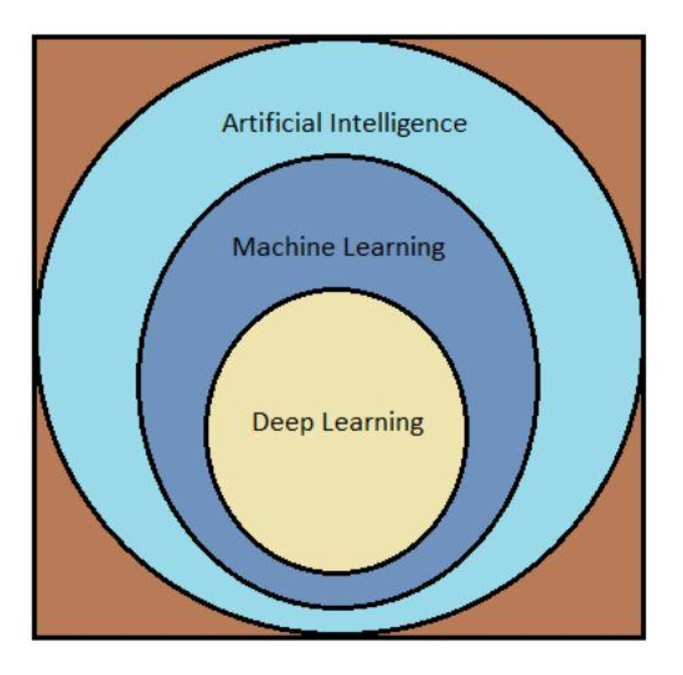
\includegraphics[width=0.4\textwidth]{images/introdl.eps}
\caption[DL vs ML vs AI]{DL vs ML vs AI. Source: Adapted from \citep{aidlml} }
\label{fig:relation}
\end{wrapfigure}

\gls{dl} is a field of AI made up of neural networks inspired by the structure and function of the human brain. AI is growing at a rapid pace and deep learning is one of the major contributors to it. Deep learning is continuously changing the world around us. Its application ranges from speech recognition to driverless cars.

Figure \ref{fig:relation} shows the relationship between DL, ML and AI.
\textbf{Artificial Intelligence} is the branch of computer science that makes the computer mimic human intelligence such as visual perception, voice recognition, translation between languages and decision making.

\textbf{Machine Learning} is the subset of AI that enables the computer to learn to do a task on its own without explicitly telling it how to accomplish the task.

\textbf{Deep Learning} is the subfield of \gls{ml}, which deals with algorithms to train models like object detection and speech recognition using a multi-layered neural network with a vast amount of data. According to \citep{lecun2015deep},
“Deep learning allows computational models that are composed of multiple processing layers to learn representations of data with multiple levels of abstraction”. 
\subsection{Neural networks}

Figure \ref{fig:snn} shows the structure of a simple neural network. An \gls{ann} usually consists of an input layer, n number of hidden layers and an output layer. The input layer receives the input and sends it to the hidden layer. The hidden layer is responsible for processing the input and extracting the features, which is then passed onto the output layer. Each layer contains several neurons, and the neurons in each layer are connected to all the neurons in the next layer. 
\begin{figure}[H]
\centering
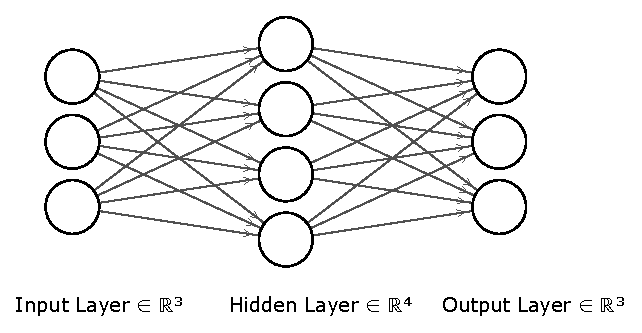
\includegraphics[width=3in]{images/nn.eps}
\caption[A simple neural network]{A simple neural network. Source: Created using tool \citep{nn}}
\label{fig:snn}
\end{figure}
\subsubsection*{Neuron}
Neurons, commonly known as nodes, are the basic building blocks of neural networks. A neuron receives input along with weights \& bias, and after processing, outputs the result as shown in Figure \ref{fig:Components of a neuron}. The output of a neuron is either used as the input to neuron in the next layer, or as the final output. 
\begin{figure}[H]
\centering
\includegraphics[width=4in,scale=1]{images/neuron.jpg}
\caption[Components of a neuron]{Components of a neuron. Source: \citep{neuron}}
\label{fig:Components of a neuron}
\end{figure}	
The output of a neuron can be mathematically represented as 
\begin{equation*}
Y=\sum_{j=1}^{n}w_{j}*x_{j} + b
\end{equation*}
	where w is the weight and b is the bias 	


\subsubsection*{Weights}

When the input data is passed into the neuron, a random weight is assigned to each information, and then the input information is multiplied by the corresponding weight. During training, the weight of each information is updated according to the corresponding feedback. 

\subsubsection*{Bias}

Bias is used as a constant to adjust the output along with the weighted sum of input in order to best fit the given data. It is added along with the result of the product of inputs and weights in the network. 

\subsubsection*{Activation function}
      The activation function converts an input signal of the neuron into any desired output signal. It is introduced to bring non-linearity into the network. The most common activation functions are sigmoid, \gls{relu}, tanh and softmax which are shown in Figure \ref{fig:activation functions}. 
\begin{figure}[H]
\centering
\includegraphics[width=4in,scale=1]{images/activation.png}
\caption[Different activation functions]{Different activation functions. Source: \citep{activation}}
\label{fig:activation functions}
\end{figure}
The final output of a neuron is given by
\begin{equation*}
      Y=\phi(\sum_{j=1}^{n}w_{j}*x_{j} + b)
\end{equation*}	
where $\phi$ can be any of these activation functions.

\subsection{Loss function and optimizer}
When training a neural network, the goal is to make the prediction as close as possible to the ground truth. The accuracy of the network is measured using the loss function. One of the most commonly used loss function is Mean Square Error (MSE). During training, the network makes use of loss value to adjust the weights so that the error is reduced at each iteration. 

\begin{equation*}
      MSE =\sum_{n}(y - \widehat{y})^2
\end{equation*}

where y is the ground truth and $\widehat{y}$ is the predictions.
\newline

	Optimizers are used to minimize the error calculated from the loss function. The most common optimization algorithm is gradient descent. \cite{kingma2014adam} proposed \gls{adam} optimizer which is the current benchmark optimizer for training deep learning models. It combines the Adagrad and RMSProp algorithm for better computational efficiency and memory requirements.

\subsection{Backpropagation}

The weights and biases in a neural network are learnable parameters. At first, when the neural network is built, they are randomly initialized. At each iteration, the network error is calculated by the forward propagation, and then to minimize the error, the gradients of the loss function are calculated and fed back to the network to update the weights \& biases in the network. This is called backpropagation.

\subsection{Hyperparameters}
 	Hyperparameters are the parameters that are not learnable during training a neural network. Some of the most common hyperparameters in deep learning are
\begin{enumerate}[(i)]
\item \textbf{Learning rate:} It is denoted by $\alpha$ that determines how fast the algorithm converges. If the learning rate is too high, it will overshoot the minima and if it is very low, the convergence will need more steps. Ideally, the learning rate is set between 0.0001 to 0.01.
\item \textbf{Regularization:} Regularization is the technique to avoid the overfitting of the model. The regularization parameter is denoted by $\lambda$. Dropout is used as a regularizer in neural networks. It refers to the training process of discarding a certain number of neurons present in the hidden layers of the network.
\begin{figure}
\centering
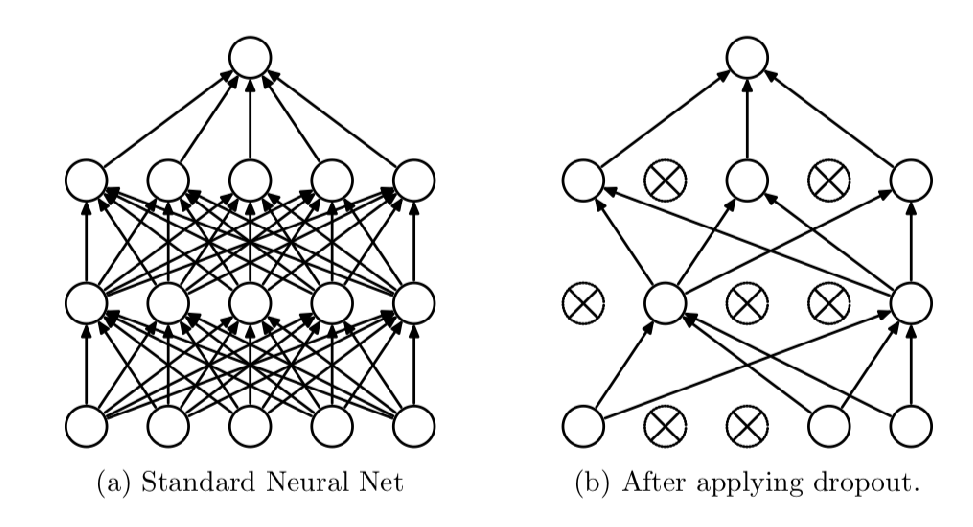
\includegraphics[width=4in,scale=1]{images/dropout.eps}
\caption[Effect of dropout]{Effect of dropout. Source: \citep{srivastava2014dropout}}
\label{fig:Dropout}
\end{figure}
\item \textbf{Batch size:} While training the neural network, instead of sending the entire input at once, the input is divided into several blocks of equal size called batches. In simple words, batch size determines the number of training examples present in a batch.
\item \textbf{Epoch:} An epoch is when the entire training data is propagated forward and backward through the neural network once.
\end{enumerate}

\section{Convolution Neural Networks}
\gls{cnn} is a type of deep neural network that is most commonly used for image recognition and classification. CNNs have been proven successful in various computer vision tasks like object detection, traffic sign detection, face recognition, scene text recognition, etc. The hidden layers \citep{Goodfellow-et-al-2016} in the CNN can be divided into convolutional layers, pooling layers, ReLU layers and fully connected layers as shown in Figure \ref{fig:cnn}.
\newline
\begin{figure}[H]
\centering
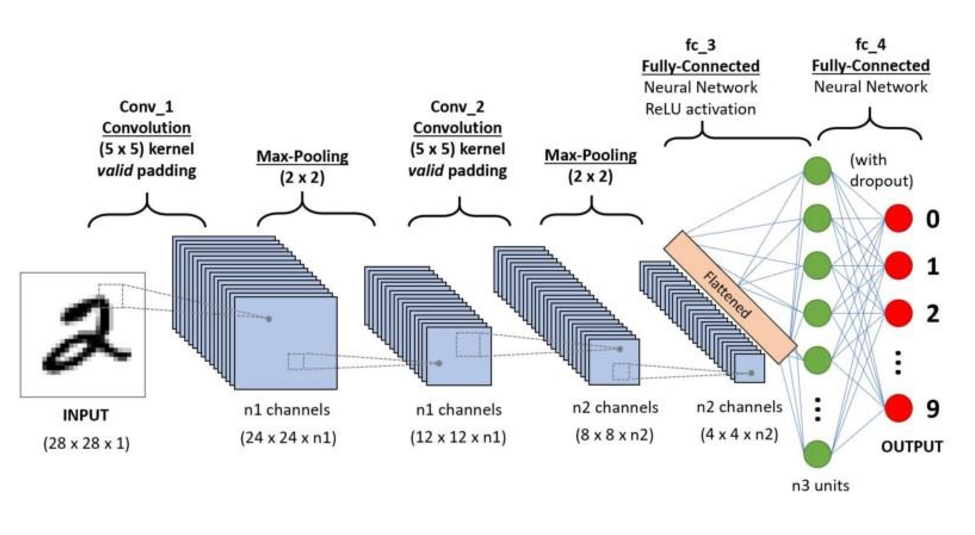
\includegraphics[width=4in,scale=1]{images/CNN.eps}
\caption[A CNN for MNIST handwritten recognition]{A CNN for MNIST handwritten recognition. Source: \citep{cnn}}
\label{fig:cnn}
\end{figure}

\subsection*{Convolution}

The operation of convolution layer starts with a kernel filter, which is just a small weight matrix. The kernel slides on the input data, multiplies the elements of the current input, and then summarizes the results into a single output pixel. The kernel repeats this process for each position in the image it slides over, transforming the input matrix into another feature matrix. The kernel filter values are randomly initialized and learnt during training.
\newline	
\begin{figure}[H]
\centering
\includegraphics[width=3in,scale=.75]{images/convolution.png}
\caption[Convolution operation]{Convolution operation. Source: \citep{convolution}}
\label{fig:convolution}
\end{figure}
Generally, an image has a shape of C x H x W where C is the number of channels of an image(for RGB, C=3), H and W are the height and width of the image. The CNN layer consists of a kernel or a filter K with x rows, y columns and depth d. The result of the convolution \citep{cnneqn} of an image I with a kernel K with d channels is given by

\begin{equation*}
Conv(I,K)\textsubscript{xy}=\sum_{i=1}^{h}\sum_{j=1}^{w}\sum_{k=1}^{d}k_{ijk}.I_{x+i-1,y+j-1,k}
\end{equation*}
\subsection*{Pooling}
After the filter passes through the image, a feature map is generated for each filter. These functions are then obtained through activation functions, which determine whether a feature exists at a given location in the image. Then we can do a lot of things, such as adding more filter layers and creating more feature maps. As we create deeper CNNs, these maps become more and more abstract. We can also use pooling layers to select the maximum values or average values on the feature map and use them as input for subsequent layers.
\newline	
\begin{figure}[H]
\centering
\includegraphics[width=3in,scale=.75]{images/maxpooling.png}
\caption[Pooling operation]{Pooling operation. Source: \citep{cnn}}
\label{fig:pooling}
\end{figure}

\subsection*{Fully connected layer}
This layer is similar to the conventional neural network, and its role is to fully connect the features obtained through multiple convolutional layers and multiple pooling layers and calculate the final predicted value. As the name implies, each neuron in this layer will be connected to all the nodes in the previous layer.
\subsection*{Normalization layer}
The normalization layer is used to normalize the activations in a neural network to give them a mean of 0 and a variance of 1. This thesis utilizes three normalization techniques i) Batch normalization, ii) Instance normalization and iii) Spectral normalization. 
\begin{enumerate}
\item \textbf{Batch normalization:} Generally the data should be normalized to make its distribution consistent. But during the training process of the deep neural networks, the data is fed into the network as batches and each batch has a different distribution. Hence \cite{ioffe2015batch} proposed batch normalization to make the distribution consistent and to reduce internal covariate shift.
\begin{figure}[H]
\centering
\includegraphics[width=4in,scale=1]{images/bnn.png}
\caption[Batch normalization algorithm]{Batch Normalization algorithm. Source: \citep{ioffe2015batch} }
\label{fig:bn}
\end{figure}
\item \textbf{Instance normalization:} The batch normalization doesn’t work well in distributed training in the case of multiple \gls{gpu}. Also, it focuses on normalizing each batch to ensure consistent data distribution. However, in image stylization, the generation result mainly depends on an image instance, so normalizing the entire batch is not suitable for image stylization. Hence, \cite{ulyanov2016instance} proposed instance normalization method normalizes only the height and width of the image. Thus it can accelerate model convergence and maintain independence between each image instance.
\begin{figure}[H]
\centering
\hspace*{1cm}\includegraphics*[width=5in,scale=1]{images/instancenorm.png}
\label{fig:ins}
\end{figure}
where x ∈ $\mathbb{R}$\textsuperscript{T×C×W×H} is the input tensor with a batch of T images and x\textsubscript{tijk} is its tijk-th element, where j and k are the dimensions, i is the feature/color channel and t is the image index in the batch \citep{ulyanov2016instance}.

\item \textbf{Spectral normalization:}
To improve the training stability of the discriminators and mitigate the problem of gradient explosion, \cite{miyato2018spectral} proposed a method called spectral normalization. It normalizes the weight for each layer of the network such that its Lipschitz constant always stays equals to one.
\end{enumerate}	

\section{Generative Adversarial Networks}
\cite{goodfellow2014generative} proposed GANs which is a type of deep neural network that generates data close to the input data distribution. The GAN network consists of two networks, Generator G and Discriminator D. These two neural networks compete against each other to learn the probability distribution of the dataset. The generator network learns to produce realistic samples and the discriminator learns to distinguish real data and samples produced from the generator. 
\begin{figure}[H]
\centering
\includegraphics[width=5in]{images/GAN.jpg}
\caption[Generative Adversarial Network (GAN)]{Generative Adversarial Network (GAN). Source: \citep{gans}}
\label{fig:gan}
\end{figure}


In Figure \ref{fig:gandist}, the black dotted line is the Gaussian distribution of real data, the green line is the fake distribution learned by the network, the blue line is the probability of judging the network as a real picture, the horizontal line marked x represents the sample following the Gaussian distribution x space, and the horizontal line marked z represents the sampling space subject to uniform distribution z. It can be seen that the mapping relationship from the space of z to the space of x is learned.
\begin{figure}[H]
\centering
\includegraphics[width=5in,scale=1]{images/GANdist.png}
\caption[Illustration of GAN learning to map uniform noise to the Gaussian distribution]{Illustration of GAN learning to map uniform noise to the Gaussian distribution. source: \citep{gandist}}
\label{fig:gandist}
\end{figure}

The training process involves two objectives
\begin{itemize}
\item The discriminator tries to maximize the probability of identifying real data from the fake data generated by the generator.
\item The generator generates realistic samples to fool the discriminator i.e. the generator tries to minimize the discriminator's probability of classifying real data from the fake data.
Thus the generator and discriminator play a minimax game.
\end{itemize}
 Both networks compete to get better against each other. The objective function V(G,D) of minimax game \citep{goodfellow2014generative} between Discriminator D and Generator G is given by
\begin{equation*}
\underset{G}{min}\underset{D}{max}V(D,G)=\mathbb{E}_{x\sim P_{data}(x)}[log D(x)] + \mathbb{E}_{z\sim P_{z}}(z)[log(1-D(G(z))]
\end{equation*}
where, D(x) is the discriminator's probability estimate that the real instance of the image is real, $\mathbb{E}_x$ is the expected value over instances of real data x, G(z) is the generator's output for the noise z, D(G(z)) is the discriminator's probability estimate that a fake instance of the image is real and $\mathbb{E}_z$ is the expected value over all random noise inputs to the generator.

\section{Conditional GANs}
	Conditional GAN is an extension of the original GAN. Both the generator and the discriminator add additional information y as a condition, y can be any information, such as class labels, image, or music data. The conditional GANs are used in various applications such as image-to-image translation, style transfer, text to image synthesis, etc.
\newline
\begin{figure}[H]
\centering
\includegraphics[width=5in]{images/cgan.jpg}
\caption[Conditional GAN]{Conditional GAN. Source: \citep{gans}}
\label{fig:cgan}
\end{figure}	
	
	 Figures \ref{fig:gan} and \ref{fig:cgan} show the difference between the standard GAN and conditional GAN ie. conditional GAN is realized by sending additional information y to the discriminator and the generator as part of the input layer. Similarly, the objective function of conditional GAN is a two-player minimax game with conditional probability \citep{isola2017image} which is given by
\begin{equation*}
\underset{G}{min} \underset{D}{max} V(D,G)=\mathbb{E}_{x\sim P_{data}(x)} [log D(x|y)] + \mathbb{E}_{z\sim P_{z}}(z) [log(1-D(G(z|y))]
\end{equation*}
where,
$D(x|y)$ is the discriminator's probability estimate that real data instance x is real given the target label y and $G(z|y)$ is the generator's output when given noise z and the target label y.
\section{OCR}
OCR is the computer vision task of localizing and detecting the text in an image. The recent developments in the deep learning approaches revived interests in the OCR problem. Different neural network architectures have been investigated to address the OCR challenge. Before the deep learning era, traditional approaches adopted connected component analysis or sliding window approaches as a solution for OCR. 
\begin{figure}[H]
\centering
\includegraphics[width=3in,scale=1]{images/ocr.png}
\caption[Optical Character Recognition]{Optical Character Recognition. Source: \citep{ocr}}
\label{fig:neuron}
\end{figure}

The existing methods can be classified into three types:
\begin{enumerate}
\item \textbf{Text detection:} It detects \& localize all the texts in the image. Bounding box coordinates is the output of the text detection.
\item \textbf{Text recognition:} It uses the output of text detection and converts the text into a digital format.
\item \textbf{End to End approach:} They perform both detection and recognition as a single approach.
\end{enumerate} 
\section{Related works}
This section provides an overview of the literature review in several related areas of research. Some of the existing methods for OCR are reviewed under different perspectives which are as follows:
\subsection{General OCR}
	Initially, researchers tried object detection models like faster R-CNN for text detection \citep{nagaoka2017text,zhong2019anchor}. But these algorithms are not very accurate and does not perform well for scene text detection.
\newline	
	
	\cite{tian2016detecting} proposed \gls{ctpn} models utilize the idea of anchoring and \gls{rnn} for sequence labelling. The input is usually passed into the pre-trained models like VGG trained with the ImageNet dataset. The output is then passed to the Bidirectional LSTM. A fully connected layer is used as an output layer which gives the bounding box coordinates for the anchor box, text probability scores and side refinements. The detection is not good for natural scene images, such as curved text and multi-directional text (vertical text).
\newline	
	
	SegLink is proposed especially for long and multi-oriented text. It is similar to the CTPN idea, at first, all parts of the text are found, and then they are connected to form a complete text line \citep{shi2017detecting}. An improved version of the SSD-based network structure is proposed to simultaneously predict two basic elements of text line detection are: segments and links. The segment is actually a bounding box output similar to the \gls{ssd} but added with a direction which is expressed as ($x_b,y_b,w_b,h_b,\theta$) where $x_b, y_b$ represents the center of the segment, $w_b, h_b$ indicates the width and height of the segment and $\theta$ represents the rotation angle of the segment. Links are the connection of segments, i.e, the probability value of whether two boxes are of the same text. One drawback of SegLink is that it cannot detect text lines with large intervals, cannot detect curved text.
\newline
	
	\cite{zhou2017east} proposed \gls{east} uses VGG16/PVANet trained on ImageNet dataset as a feature extractor. The input is passed into the feature extractor and a U-Net architecture is used to merge the feature maps. The output layer consists of probabilities of text in a region and all the bounding box coordinates. The limitation is that the receptive field of EAST is not very large and hence it is not good for detecting lengthy texts.
\newline
	
	The existing text detection methods such as bounding box regression is not accurate for the texts in arbitrary shapes such as curved text, and the segmentation method does not work well when the text is close to each other. In order to solve these two problems, \cite{wang2019shape} proposed a new method called a new \gls{pse}. It works as a segmentation based detector with numerous predictions with for every individual text instance. Thus, the proposed pixel-based segmentation method can accurately locate texts of any shape and detect two text instances even when they are very close. 
\newline
	
	Similar to the above approach, \cite{tian2019learning} proposed a method called Learning Shape-Aware Embedding for Scene Text Detection. The idea is to map image pixels to embedding in the feature space, pixels belonging to the same text instance will be closer to each other in the space, whereas pixels of different text instances will be further away from each other. ResNet-50 is used as a feature extractor. The network output includes the embedded feature map and the mask map of texts. It performs well on three benchmark scene text detection datasets ICDAR15 \citep{icdar}, MSRA-TD500 \citep{msra}, and CTW1500 \citep{yuan2019ctw}.
\newline
	
	\cite{wang2019arbitrary} introduced a method called Arbitrary Shape Scene Text Detection with Adaptive Text Region Representation. It involves two-stage text detection. The first stage is similar to Faster R-CNN. Text proposals are obtained through \gls{cnn} + \gls{rnn} + \gls{roi}. The second stage is to refine the text proposals to make the prediction frame more accurate. The network uses SE-VGG16 as a feature extractor. Experiments show that \gls{se} Block can improve performance. The main advantage of the proposed method is that it uses adaptive points instead of fixed points to represent a text box. The previous methods used fixed points to represent the text box, but the number of points for horizontal text, multidirectional text, and curved text is not the same. So, the points to represent the text box are adapted to detect text of various shapes. It uses the \gls{lstm} network to learn how many points should be used to represent the text box.
\newline
	
	Similar to SegLink, \cite{baek2019character} proposed \gls{craft} that detects text area by identifying single character (character region score) and connection between each characters (affinity score). The network structure is similar to the EAST network structure: the feature extraction backbone network part uses VGG-16 with batch normalization; the feature decode module is similar to U-Net, and it also uses a top-down feature aggregation method; the network finally outputs two channel feature map, that is, region score map and affinity score map in the form of the heat map. This thesis uses the CRAFT pre-trained model for text detection and \cite{baek2019wrong} proposed model for text recognition.

\subsection{OCR for steel type plates}

	Similar to steel type plate recognition, many research works have been published to extract text from the vehicle license plate, forms, and documents \citep{duan2005building,zang2015vehicle,impedovo2012fundamentals,
milewski2006extraction,laroca2018robust}. Several deep learning and computer vision algorithms exist to solve these problems. But the existing approach would fail for our steel type plate images since the complexity of our problem is relatively higher. 
Before the deep learning era, there have been several classical research works done to improve the accuracy of OCR for steel type plates. Some of the approaches similar to our problem are discussed below: 
\newline
	
	\cite{novak2013recognition} used fuzzy logic methods for the recognition of distorted characters printed on metal. \cite{yu2017engraving} proposed a technique that involved image processing with a series of mathematical and morphological treatments for metal surface engraving character detection.  \cite{xiang2018metal} proposed a technique called \gls{msc}. They combined and fused the images of the steel plates of the same scene from multi-direction and different illuminations to improve the character recognition of metal stamped characters. \cite{raka2019ocr} proposed an algorithm based on \gls{knn} for reading embossed text from credit/debit cards. After preprocessing steps, they locate the credit/debit card number and split it into individual characters. They created a dataset by manually sorting characters from 0 - 9 and then trained the OCR model with its corresponding label using KNN. These classic approaches are performing basic image manipulation operations like image binarization, thresholding, segmentation and other morphological processes to increase the quality of the original image. 
\newline

	Recent advancements in computer vision have given a set of new possibilities to tackle advanced recognition problems. \cite{patil2015engraved} proposed a computer vision technique to identify texts from the engine and chassis parts.  With the success of CNNs in the image classification \citep{hinton2012improving,simonyan2014very}, Segmentation \citep{girshick2014rich}, Object Detection \citep{russakovsky2015imagenet}, it is combined with recurrent networks along with attention mechanism for solving OCR problem. 
\newline

	\cite{bui2017selecting} proposed an algorithm that automatically selects the preferred pre-processing methods to be applied to a document image to maximize OCR performance for the processed image. They used 21 different such possible combinations to pre-process the image. Their approach achieved a good improvement in the performance of OCR. But the main drawback is that the possible pre-processing options were limited. Also, it does not suit our requirements.  
\newline

	Similar to our approach, \cite{hu2019embossed} used CNN for enhancing the character recognition of embossed characters of the shoe soles. Their research focussed only on image enhancement and did not care about the character recognition part.
	
\subsection{GANs in OCR}
	 Using standard GANs, \cite{karras2017progressive} generated highly realistic human faces trained with the celebrity dataset while \cite{jin2017towards} generated faces of anime characters. Likewise, \cite{brock2018large} demonstrated the ability of GANs to generate synthetic images of objects that are not differentiable from the real images using the BigGAN technique. Works such as \citep{zhang2017stackgan,reed2016learning,reed2016generative,dash2017tac} used conditional GANs to generate images given its description as text which is popularly known as text-to-image translation.
\newline

	Large scale annotated datasets are required for the development of robust deep learning models, especially for CNN. Acquiring such datasets is always challenging in cases like medical images. Hence, \cite{frid2018gan} used GANs to generate synthetic medical images as a data augmentation technique to increase the performance of CNN in classifying images of liver lesions. Similarly, \cite{fiore2019using} used GAN for improving the effectiveness of classifying credit card fraud detection. Even though it was a binary classification problem, the dataset was heavily imbalanced i.e. the interested class was represented significantly lesser than the other. Synthetic images were generated for the imbalanced class as an alternative to oversampling techniques.
\newline
	
	For our case, since the goal was to generate a clear image from noisy steel type plate images in order to maximize the OCR performance, it was realized that one way to go about solving this problem is by using a generative adversarial image. 
Some of the research works using GANs for improving character recognition are presented below:
\newline

	\cite{hosangadi2019ocr} proposed a method that uses DCGAN for enhancing the image quality of documents to improve the OCR performance. Their model uses an encoder trained to learn the latent representation of a low-quality image. The latent representation is then passed as an input to the conditional GAN generator which is trained to produce a high-quality image.
\newline
	
	 \cite{lat2018enhancing} proposed a super-resolution based solution for improving the OCR accuracy using GAN. They used SRGAN to convert the low resolution (scanned at as low as 75dpi) document images into super-resolved texts and then passed it into the OCR engine. 
\newline
	 
	 Similarly, \cite{karimi2020illegible} developed a model called Handwritten-to-Machine-Print Generative Adversarial Network (HW2MP-GAN) to transform the handwritten text to machine-printed text. Their model utilizes sliced Wasserstein distance and U-Net architecture for better quality image-to-image translation. These approaches work well for printed documents and have shown to improve the accuracy of OCR.
\newline

	In summary, we list out the papers that especially influenced this work. The proposed overall framework uses a GAN generator model and an OCR engine. For GAN, the best generator model is selected among the three image-to-image translation GANs: i) \cite{isola2017image} proposed a pix2pix GAN , ii) \cite{CycleGAN2017} proposed CycleGAN  and iii) \cite{stoller2019training} proposed FactorGAN. For OCR engine, the text detection uses CRAFT approach \citep{baek2019character} and the text recognition uses \cite{baek2019wrong} proposed text recognition model.
\newpage
\chapter{Methodology}\label{ch:method}
This chapter describes the key idea, the proposed framework and methodology used in this thesis. A comparison between different image-to-image translation models using GANs is provided. Also, the architecture of text detection and text recognition models used for the OCR engine has been presented. This chapter discusses, in brief, each of the components used in the overall framework and their implementation procedures.
\newline

        The image-to-image translation is the class of computer vision problems where the goal is to learn the mapping between input and target domain. The applications of image-to-image translation range from style transfer, colorization, sketches to photo, and image super-resolution. In this thesis, we have investigated three different image-to-image translation GANs: Pix2pix, CycleGAN and FactorGAN to improve the readability of texts present in the steel type plate/nameplate images. Then the best generator model from the three GANs is selected and integrated with the pre-trained text detection \& text recognition model.

\section{Pix2pix GAN}
	\cite{isola2017image} proposed pix2pix (pixel to pixel) Generative Adversarial Network that has shown to produce realistic and detailed synthetic images. Pix2pix is a supervised image-to-image translation model that uses conditional GANs to learn a function to map input image to output image.  

\subsection{Architecture}
Similar to the standard GAN, the pix2pix model consists of two components i) Generator and ii) Discriminator as shown in Figure \ref{fig:pix}. The generator transforms the input image to an image in the target domain while the discriminator measures the similarity of the input image to image passed randomly either generated by generator or the real image and predicts the probability of the image being real. The pix2pix model is a type of conditional generative model with a target image as additional information. 

\begin{figure}[H]
\centering
\includegraphics[width=5in]{images/pix2pix.png}
\caption[Architecture of pix2pix]{Architecture of pix2pix. Source: Adapted from \citep{isola2017image}}
\label{fig:pix}
\end{figure}

In contrast to the standard conditional GANs, the generator takes the source image with no noise as input whereas both the source image and target image are passed to the discriminator as shown in Figure \ref{fig:pix}. The generator is trained with adversarial loss and L1 loss to produce a meaningful translation of a source image to a target image. Also, the randomness is added to the network in the form of dropout. The architecture of the generator and the discriminator is explained in detail which is as follows:

\subsubsection*{Generator}

	For the generator architecture, the ResNet framework proposed by \citeauthor{he2016deep} was used. Residual Network (ResNet) is a CNN architecture consists of a series of residual blocks with skip connections to address the problem of vanishing gradients. The vanishing gradients problem occurs in deep neural networks when the weights of the initial layer not getting updated properly during back-propagation as the repeated multiplication makes the gradient small. Thus, the performance gets saturated with more layers in the network. Apart from this problem, they showed that adding more layers to the neural network slows down the training and does not improve accuracy. ResNet uses the identity matrix via skip connection that multiplies the gradient by 1 during backpropagation. Thus, it preserves the gradient and avoids information loss \citep{he2016deep,resnet}. 

\begin{figure}[H]
\centering
\includegraphics[width=4in]{images/resnetblock.PNG}
\caption[Difference between residual block (left) vs ordinary CNN (right) connections]{Difference between residual block (left) vs ordinary CNN (right) connections. Source: Supplementary material, \citep{johnson2016perceptual}}
\label{fig:resblock}
\end{figure}

The differentiating factor of ResNet from a CNN is their skip connection which is shown in Figure \ref{fig:resblock}. The skip connection adds the original input to the output of the convolution block. In traditional CNNs, each layer output is fed as input to the next layer, but with skip connections, each layer output is passed to consecutive layers as well as the non-consecutive layers. This helps in solving the problem of vanishing gradient and the identity matrix helps in maintaining the performance of initial layers with the higher layers \citep{resnet}. In our approach, the generator accepts an input image of size 600 x 400 x 3 and generates an output image of the 600 x 400 x 1. The full generator architecture is shown in Table \ref{tab:tab1}. \\

\begin{table}[h]
\centering
\begin{tabular}{|c|c|c|c|} 
\hline
\textbf{~ Block~} & \textbf{~ Filters} & \textbf{~Filter size~} & \textbf{~Stride}  \\ 
\hline
Conv-BN-ReLU      & 64                 & 7x7                    & 1                 \\ 
\hline
Conv-BN-ReLU      & 128                & 3x3                    & 2                 \\ 
\hline
Conv-BN-ReLU      & 256                & 3x3                    & 2                 \\ 
\hline
Residual Block1   & 256                & 3x3                    & 1                 \\ 
\hline
Residual Block2   & 256                & 3x3                    & 1                 \\ 
\hline
Residual Block3   & 256                & 3x3                    & 1                 \\ 
\hline
Residual Block4   & 256                & 3x3                    & 1                 \\ 
\hline
Residual Block5   & 256                & 3x3                    & 1                 \\ 
\hline
Residual Block6   & 256                & 3x3                    & 1                 \\ 
\hline
Residual Block7   & 256                & 3x3                    & 1                 \\ 
\hline
Residual Block8   & 256                & 3x3                    & 1                 \\ 
\hline
Residual Block9   & 256                & 3x3                    & 1                 \\ 
\hline
ConvT-BN-ReLU     & 128                & 3x3                    & 2                 \\ 
\hline
ConvT-BN-ReLU     & 64                 & 3x3                    & 2                 \\ 
\hline
Conv-tanh         & 1                  & 7x7                    & 1                 \\
\hline
\end{tabular}
\caption{Architecture of pix2pix generator}
\label{tab:tab1}
\end{table}
The generator consists of encoder, 9 ResNet blocks and decoder blocks. Each encoder and decoder block consists of a convolution layers, a batch normalization (BN) layer followed by the ReLU activation function. Each ResNet block has two connections from its input, one connection going through a series of convolutions, batch normalization \& activation functions and the other connection skipping over that series as shown in the Figure \ref{fig:resblock}.

\subsubsection*{Discriminator}

The PatchGAN architecture proposed by \cite{li2016precomputed} was used for the discriminator. It compares NxN patches of the image instead of the entire image to classify if it is real or fake. Thus, the PatchGAN is more suitable for producing sharp high-frequency detail and have shown great classification performance in GANs. We used the default 70 x 70 patches as suggested in the pix2pix paper. The discriminator architecture is shown in Table \ref{tab:tab2}. Here LReLU represents the Leaky ReLU activation function.

\begin{table}[H]
\centering
\begin{tabular}{|c|c|c|c|} 
\hline
\textbf{Block~}        & \textbf{Filters} & \textbf{Filter size~} & \textbf{Stride}  \\ 
\hline
Conv-LReLU~~           & 64               & 4x4                   & 2                \\ 
\hline
Block 2 Conv-BN-LReLU~ & 128              & 4x4                   & 2                \\ 
\hline
Block 3 Conv-BN-LReLU~ & 256              & 4x4                   & 2                \\ 
\hline
Block 4 Conv-BN-LReLU~ & 512              & 4x4                   & 1                \\ 
\hline
Block 5 Conv-Sigmoid~  & 1                & 4x4                   & 1                \\
\hline
\end{tabular}
\caption{Architecture of pix2pix discriminator}
\label{tab:tab2}
\end{table}

It consists of 5 blocks of convolution layers. The Leaky ReLU with 0.2 negative slope is used as an activation function. The first convolutional layer consists of 64 filters and it is upscaled after each block. At the final layer, a sigmoid activation function is used to predict if the 70 x 70 patch image is real or fake.

\subsection{Loss function}
The loss function of the pix2pix is the same as the conditional GAN as discussed in the earlier section. The $L_1$ loss is added extra to the loss function since the goal of the generator is to generate realistic images such that it fools the discriminator. The $L_1$ loss calculates the pixel-wise difference between the source image and the target image. Thus forcing the generator to produce images close to the ground truth. The adversarial loss \citep{isola2017image} is given by
\begin{equation*}
L\textsubscript{adv}(G,D)=\mathbb{E}_{x,y}[log D(x,y)] + \mathbb{E}_{x,z}[log(1-D(x,G(x,z))]
\end{equation*}
The $L_1$ loss \citep{isola2017image} is given  by 
\begin{equation*}
L\textsubscript{L1}(G)=\mathbb{E}_{x,y,z}[\lVert y - G(x,z) \rVert_1]
\end{equation*}
And the final objective function \citep{isola2017image} is the sum of the adversarial loss and the $L_1$ loss which is given  by

\begin{equation*}
G^*=arg\underset{G}{min}\underset{D}{max}L\textsubscript{adv}(G,D)\; + \;\lambda L\textsubscript{L1}(G)
\end{equation*}
\noindent
where $\lambda$ is the scalar used to determine the importance of the $L_1$ loss.

\section{CycleGAN}
CycleGAN is an unsupervised method for training image-to-image translation models. They learn the characteristics and styles from an image collection of the source domain and translates it to the target domain in the absence of paired data. \\
\begin{wrapfigure}{r}{0.6\textwidth}
\centering
\includegraphics[width=0.5\textwidth]{images/newcyc.png}
\caption[Paired \& unpaired datasets]{Paired \& unpaired datasets. Source: Adapted from \citep{CycleGAN2017}}
\label{fig:pau}
\end{wrapfigure}
	The need for one to one mapping is eliminated by transforming the image from the source domain to the target domain and then back to the source domain just like translating a sentence from English to German and from German to English. 
\newline

	The authors conducted experiments on various image datasets such as horse $\leftrightarrow$ zebra, apple $\leftrightarrow$ orange, photo $\leftrightarrow$ monet, etc. Relaxing the one to one mapping makes the CycleGAN a more powerful method to tackle a variety of problems like the translation of noisy steel type plate images to clear images.

\subsection{Architecture}

Every image in a paired dataset is manually mapped from domain X to domain Y. Thus images in both domains share some common features. This pairing defines a meaningful relationship between images in both domains. In pix2pix, the generator takes input from domain X and translates it to an image close to domain Y. The CycleGAN with an unpaired dataset does not have this luxury since there is no meaningful transformation that it can learn.
The difference between the paired and unpaired dataset is shown in Figure \ref{fig:pau}. To establish a meaningful relationship in the unpaired dataset, \citeauthor{CycleGAN2017} introduced the concept of cycle consistency. The cycle consistency refers to the ability of translating an image from domain X to domain Y and then the generated image is translated back again to domain X. The architecture of CycleGAN is shown in Figure \ref{fig:cycarch}.

\begin{figure}[H]
\centering
\includegraphics[width=5in]{images/cycGANarch.PNG}
\caption[Architecture of CycleGAN]{Architecture of CycleGAN. Source: Adapted from \citep{CycleGAN2017}}
\label{fig:cycarch}
\end{figure}

A generator will map the input image from a source domain to some image in the target domain with a constraint that the generated image must share some features that can map back to its original image. Thus the CycleGAN architecture consists of two generators G and F. The goal of generator G is to map X domain to Y domain such that G: X\textrightarrow Y and the other generator F will map Y domain to X such that F: Y\textrightarrow X. These generators have their respective discriminators $D_x$ and $D_y$. Discriminator $D_x$ forces generator G to translate images from domain X into an output that is indistinguishable from the images of domain Y and vice versa for Discriminator $D_y$.

\subsubsection*{Generator}
The same ResNet-9 blocks discussed in the pix2pix section was used as the architecture for both generators. Since the two generators are used, the images are resized to 300 x 300 to adapt to the memory requirements of the system. The instance normalization is replaced by batch normalization since multiple GPUs are used for training. The full generator architecture is explained in detail in Table \ref{tab:tab3}.

\begin{table}[H]
\centering
\begin{tabular}{|c|c|c|c|} 
\hline
\textbf{Block~} & \textbf{Filters} & \textbf{Filter size~} & \textbf{Stride}  \\ 
\hline
Conv-IN-ReLU    & 64               & 7x7                   & 1                \\ 
\hline
Conv-IN-ReLU    & 128              & 3x3                   & 2                \\ 
\hline
Conv-IN-ReLU    & 256              & 3x3                   & 2                \\ 
\hline
Residual Block1 & 256              & 3x3                   & 1                \\ 
\hline
Residual Block2 & 256              & 3x3                   & 1                \\ 
\hline
Residual Block3 & 256              & 3x3                   & 1                \\ 
\hline
Residual Block4 & 256              & 3x3                   & 1                \\ 
\hline
Residual Block5 & 256              & 3x3                   & 1                \\ 
\hline
Residual Block6 & 256              & 3x3                   & 1                \\ 
\hline
Residual Block7 & 256              & 3x3                   & 1                \\ 
\hline
Residual Block8 & 256              & 3x3                   & 1                \\ 
\hline
Residual Block9 & 256              & 3x3                   & 1                \\ 
\hline
ConvT-IN-ReLU   & 128              & 3x3                   & 2                \\ 
\hline
ConvT-IN-ReLU   & 64               & 3x3                   & 2                \\ 
\hline
Conv-tanh       & 1                & 7x7                   & 1                \\
\hline
\end{tabular}
\caption{Architecture of CycleGAN generator}
\label{tab:tab3}
\end{table}

\subsubsection*{Discriminator}
The PatchGAN discussed in the pix2pix section was used as the architecture for both the discriminators with the default setting 70 x 70. The full discriminator architecture is explained in detail in Table \ref{tab:tab4}.

\begin{table}[H]
\centering
\begin{tabular}{|c|c|c|c|} 
\hline
\textbf{Block~}        & \textbf{Filters} & \textbf{Filter size~} & \textbf{Stride}  \\ 
\hline
Conv-LReLU~~           & 64               & 4x4                   & 2                \\ 
\hline
Block 2 Conv-IN-LReLU~ & 128              & 4x4                   & 2                \\ 
\hline
Block 3 Conv-IN-LReLU~ & 256              & 4x4                   & 2                \\ 
\hline
Block 4 Conv-IN-LReLU~ & 512              & 4x4                   & 1                \\ 
\hline
Block 5 Conv-Sigmoid~  & 1                & 4x4                   & 1                \\
\hline
\end{tabular}
\caption{Architecture of CycleGAN discriminator}
\label{tab:tab4}
\end{table}

\subsection{Loss function}

	The loss function of CycleGAN needs to satisfy the following condition - i.e., the generated image should always be mapped back to its original image.
\newline

	Let the two generators be G, F and two discriminators $D_x$, $D_y$. The goal of the generators is to translate an image from domain X to Y and vice versa. Let the training samples in the domain X is defined as $\{x_i\}_{i=1}^N$ and training samples in the domain Y is defined as $\{y_j\}_{i=1}^M$. The distribution of the data is defined as the $x\sim p_{data}(x)$ and $y\sim p_{data}(y)$. The loss function of CycleGAN is defined by two losses: i) Adversarial loss and ii) Cycle consistency loss.
\newline

	The adversarial loss is used to match the distribution of generated images with the target domain. It is applied to both the generators. The adversarial loss \citep{CycleGAN2017} for generator G that translates the image from domain X to domain Y such that G: X\textrightarrow Y is given by
\begin{equation*}
L\textsubscript{GAN} (G,D_Y,X,Y)=\mathbb{E}_y\sim p_{data}(y)[log D_Y(y)] \; + \; \mathbb{E}_x\sim p_{data}(x)[log(1-D_Y(G(x))]
\end{equation*}
Likewise for generator F that translates the image from domain Y to domain X such that F: Y\textrightarrow X is given by,
\begin{equation*}
L\textsubscript{GAN}(F,D_X,Y,X)=\mathbb{E}_x\sim p_{data}(x)[log D_X(x)] \; + \; \mathbb{E}_y\sim p_{data}(y)[log(1-D_X(F(y))]
\end{equation*}

The cycle consistency loss enables both the generators to be stable and consistent. This loss regulates the GAN training process and makes sure that the generator does not generate any random permutation of images in the target domain \citep{CycleGAN2017}. It is given by

\begin{equation*}
L\textsubscript{cyc}(G,F)=\mathbb{E}_{x\sim p_{data}(x)}[\lVert F(G(x)) \; - \; x \rVert_1] \; + \; \mathbb{E}_{y\sim p_{data}(y)}[\lVert G(F(y)) - y \rVert_1]
\end{equation*}

Combining these two losses, 	
\begin{equation*}
L\textsubscript{GAN}\;(G,F,D_X,D_Y) = L\textsubscript{GAN}\;(G,D_Y,X,Y) \;+ \;L\textsubscript{GAN}\;(F,D_X,Y,X) \;+\; \lambda L\textsubscript{cyc}(G,F)
\end{equation*}
where $\lambda$ controls the importance of cycle consistency loss. So, the final objective function \citep{CycleGAN2017} is given by
\begin{equation*}
G^*,F^*=arg\underset{G,F}{min}\underset{D_X,D_Y}{max}L(G,F,D_X,D_Y)
\end{equation*}

\section{FactorGAN}
The last GAN that is investigated in this thesis is \cite{stoller2019training} proposed FactorGAN. Even though the GANs have been producing realistic images with greater success, they rely heavily on the amount of training data. Even though the datasets for the everyday objects are widely available, the datasets for specific industrial use case remains scarce. In the case of pix2pix, the generation of image pairs is time consuming, requires a lot of manual annotation and is expensive. The CycleGAN model does not make use of the paired information in the dataset. Although the methods like \citep{tripathy2018learning,almahairi2018augmented} use both the information of paired and unpaired data with additional reconstruction losses, they have to be balanced with many hyperparameters. This leads to computational overheads and thus the convergence of the generator to the desired distribution becomes uncertain \citep{stoller2019training}. The FactorGAN provides a solution to enable training for generative models with incomplete observations ie when the paired data is less.
\begin{figure}[H]
\centering
\includegraphics[width=5in]{images/factorgan.PNG}
\caption[Architecture of FactorGAN]{Architecture of FactorGAN. Source: Adapted from \citep{factgit}}
\label{fig:factorgan}
\end{figure}
\subsection{Architecture}
The FactorGAN uses a generator and three discriminators as shown in Figure \ref{fig:factorgan}. The generator generates a clear image of the steel type plate close to the target domain while the discriminator classifies the real and fake image. A real dependency discriminator distinguishes the real steel type plates and its ground truth pairs. A fake dependency discriminator distinguishes the real steel type plates and generated image pairs. 
\begin{figure}
\centering
\includegraphics[width=5in]{images/unet.PNG}
\caption[Architecture of U-Net]{Architecture of U-Net. Source: \citep{ronneberger2015u}}\label{fig:unet}
\end{figure}
\subsubsection*{Generator}
The U-Net architecture proposed by \cite{ronneberger2015u} was used for the generator model. U-Net is a fully convolutional neural network that can be composed into three parts: shrinkage, bottleneck and expansion. It consists of conv layers, max pooling, ReLU activation, concatenation layers, up and down sampling as in Figure \ref{fig:unet}. The shrinkage part on the left uses convolution and max pooling operations. The expansion part on the right uses several blocks with upsampling and concatenation \citep{ronneberger2015u}. The full generator architecture is shown in Table \ref{tab:tab5}.
\begin{table}[H]
\centering
\begin{tabular}{|c|c|c|c|} 
\hline
\textbf{Block~} & \textbf{Filters} & \textbf{Filter size~} & \textbf{Stride}  \\ 
\hline
Conv-BN-ReLU    & 32               & 3x3                   & 1                \\ 
\hline
Conv-BN-ReLU    & 32               & 3x3                   & 1                \\ 
\hline
Conv-BN-ReLU    & 64               & 3x3                   & 1                \\ 
\hline
Conv-BN-ReLU    & 64               & 3x3                   & 1                \\ 
\hline
Conv-BN-ReLU    & 128              & 3x3                   & 1                \\ 
\hline
Conv-BN-ReLU    & 128              & 3x3                   & 1                \\ 
\hline
Conv-BN-ReLU    & 256              & 3x3                   & 1                \\ 
\hline
Conv-BN-ReLU    & 256              & 3x3                   & 1                \\ 
\hline
Conv-BN-ReLU    & 256              & 3x3                   & 1                \\ 
\hline
Conv-BN-ReLU    & 256              & 3x3                   & 1                \\ 
\hline
Conv-BN-ReLU    & 128              & 3x3                   & 1                \\ 
\hline
Conv-BN-ReLU    & 128              & 3x3                   & 1                \\ 
\hline
Conv-BN-ReLU    & 64               & 3x3                   & 1                \\ 
\hline
Conv-BN-ReLU    & 64               & 3x3                   & 1                \\ 
\hline
Conv-BN-ReLU    & 32               & 3x3                   & 1                \\ 
\hline
Conv-BN-ReLU    & 32               & 3x3                   & 1                \\ 
\hline
Conv-BN-ReLU    & 32               & 3x3                   & 1                \\ 
\hline
Conv-BN-ReLU    & 32               & 3x3                   & 1                \\ 
\hline
Conv-sigmoid    & 1                & 1x1                   & 1                \\
\hline
\end{tabular}
\caption{Architecture of FactorGAN generator}
\label{tab:tab5}
\end{table}

\subsubsection*{Discriminator}
The architecture of the discriminator is shown in Table \ref{tab:tab6}. It consists of convolution layers with spectral normalization and LReLU activation. All the layers except the fully convolution layer have biases. Spectral normalization normalizes the weight such that the Lipschitz constant for each layer as well as the whole network is one.
\begin{table}[H]
\centering
\begin{tabular}{|c|c|c|c|} 
\hline
\textbf{Block~}        & \textbf{Filters} & \textbf{Filter size~} & \textbf{Stride}  \\ 
\hline
Conv-SN                & 32               & 4x4                   & 2                \\ 
\hline
Block 2 Conv-SN-LReLU~ & 64               & 4x4                   & 2                \\ 
\hline
Block 3 Conv-SN-LReLU~ & 128              & 4x4                   & 2                \\ 
\hline
Block 4 Conv-SN-LReLU~ & 256              & 4x4                   & 2                \\ 
\hline
Block 5 Conv-SN-LReLU~ & 512              & 4x4                   & 2                \\ 
\hline
Block 6 Conv-SN-LReLU~ & 1024             & 4x4                   & 2                \\ 
\hline
Block7 Conv-LReLU      & 1                & 1x1                   & 1                \\
\hline
\end{tabular}
\caption{Architecture of FactorGAN discriminator}
\label{tab:tab6}
\end{table}

\subsection{Objective function}
Let the probability distribution of a dataset is $p_x$ over $x \in \mathbb{R}^d$, discriminator $D_\theta$ and the generator be $G_\phi$ that maps an n dimensional input $z \sim p_z$ to a d dimensional sample $g_\phi(z)$ resulting in the generator distribution $q_x$. Then the loss function \citep{stoller2019training} for standard GAN is given by

\begin{equation*}
arg\underset{\theta}{max}\;\mathbb{E}_{z\sim p_{z}} log D_\theta(G_\phi(z))
\end{equation*}	

To train the GAN with incomplete observation \citep{stoller2019training}, the discriminator D is mapped to a joint density ratio $\frac{p_x(x)}{q_x(x)}$. This joint density ratio is factorized into a product of density ratios.
\begin{align*}
h(\widetilde{D}(x)) = \frac{p_x(x)}{q_x(x)} = \frac{c_P(x)}{c_Q(x)}\prod_{i=1}^{K}\frac{p_x^i(x^i)}{q_x^i(x^i)}\;\;\text{where,}\\c_P(x)= \frac{p_x(x)}{\prod_{i=1}^{K}p_x^i(x^i)}\text{\;\&}\; c_Q(x)= \frac{q_x(x)}{\prod_{i=1}^{K}q_x^i(x^i)}
\end{align*}

For conditional GAN \citep{stoller2019training}, the generator $g_\phi$ that maps a conditional input $x^1$ and a noise to an output $x^2$ resulting in output probability $q_\phi(x^2|x^1)$. In order to eliminate the need for the paired samples, applying the factorization to $x^1$ and $x^2$ with K=2 in the above equation results in 

\begin{equation*}
\frac{p_x(x)}{q_x(x)} = \frac{\frac{p_x(x)}{p_x^1(x^1)p_x^2(x^2)}}{\frac{q_x(x)}{q_x^1(x^1)q_x^2(x^2)}} = \frac{c_P(x)}{c_Q(x)}\frac{p_x^2(x^2)}{q_x^2(x^2)}
\end{equation*}	


From the above equation, \citeauthor{stoller2019training} justified the use of p and q dependency discriminator to model the input-output relationship and a marginal discriminator.
\newline 


\section{Comparison of image-to-image translation GANs under study}
	To summarize, Table \ref{tab:tab7} presents a brief comparison of the above discussed image-to-image translation GANs. The networks describe the complexity of the model with number of generators and discriminators present. Image size denotes the size of input in pixels used in each GAN. Release date is the given publication date for each related article. The method, backbone, normalization and type represent the loss function, architecture, type of normalization and learning approach used for each GAN respectively. 
\begin{table}[H]
\resizebox{\textwidth}{!}{%
\begin{tabular}{|c|c|c|c|}
\hline
                       & \textbf{Pix2pix}           & \textbf{CycleGAN}      & \textbf{FactorGAN}        \\ \hline
\textbf{Method}        & Adversarial loss + L1 loss & Cycle consistency loss & Factorized discriminators \\ \hline
\textbf{Networks} &
  \begin{tabular}[c]{@{}c@{}}1 Generator\\ 1 Discriminator\end{tabular} &
  \begin{tabular}[c]{@{}c@{}}2 Generators \\ 2 Discriminators\end{tabular} &
  \begin{tabular}[c]{@{}c@{}}1 Generator \\ 1 Marginal Discriminator \\ 2 Dependency Discriminators\end{tabular} \\ \hline
\textbf{Image size}    & 600 x 400                  & 300 x 300              & 256 x 256                 \\ \hline
\textbf{Release date}  & 2017 - 2018                & 2017 - 2018            & 2019 - 2020               \\ \hline
\textbf{Normalization} & Batch                      & Instance               & Spectral                  \\ \hline
\textbf{Backbone}      & ResNet                     & ResNet                 & U-Net                      \\ \hline
\textbf{Type} &
  \begin{tabular}[c]{@{}c@{}}Supervised method that\\ requires paired dataset\end{tabular} &
  \begin{tabular}[c]{@{}c@{}}Unsupervised method that\\ requires unpaired dataset\end{tabular} &
  \begin{tabular}[c]{@{}c@{}}Semi-supervised method \\ that handles incomplete\\  data points\end{tabular} \\ \hline
\end{tabular}%
}
\caption{Comparison of image-to-image translation GANs under study}
\label{tab:tab7}
\end{table}
\section{OCR - Text detection}
\cite{baek2019character} proposed Character Region Awareness For Text detection (CRAFT) is the state of the art for scene text detection. We have used the pre-trained model trained using the CRAFT approach in this thesis for text detection.
\newline

	When the problem of text detection is applied to real-world scenarios, it can be seen that the texts in the real world are curved, arbitrary or in an irregular shape. The existing bounding box-based method implemented using the anchor box cannot handle the scenarios where the text is excessively deformed or the text is too large. To improve the text detection in such scenarios, the CRAFT framework was proposed.
\begin{figure}[H]
\centering
\includegraphics[width=5.5in]{images/craft.jpg}
\caption[The process of CRAFT]{The process of CRAFT: (a) Input image (b) Character region map (c) Affinity score map (d) Text detection output. Source: Adapted from \citep{craft}}
\label{fig:craft}
\end{figure}
The idea of CRAFT is to detect text by exploring each character region and affinity between the characters. It first locates each character in the word using the region score. Then predict whether each character belongs to the same text using the affinity score and concatenate. Thus this model mainly outputs two things:

\begin{enumerate}[(i)]
\item\textbf{Region score} gives the probability of the detected location being a character.
\item\textbf{Affinity score} gives the probability of whether the character at this position needs to be concatenated into a word.
\end{enumerate}


\begin{figure}[H]
\centering
\includegraphics[width=5in]{images/craftarch.png}
\caption[The CRAFT architecture]{The CRAFT architecture. Source: \citep{baek2019character}}
\label{fig:craftarch}
\end{figure} 

The network structure of the CRAFT is shown in Figure \ref{fig:craftarch}. The backbone network is VGG-16, followed by the feature fusion of Feature Pyramid Network. The final output of the model generates a character region prediction (region score) and character association prediction (affinity score). Since the existing datasets for training the text detection models are based on word-level annotations and there is no character level labelling, \citeauthor{baek2019character} used synthetic character dataset for training. The pre-trained model used in this thesis is trained in SynthText \citep{Gupta16}, ICDAR13, ICDAR17 datasets.

\section{OCR - Text recognition}

Several different methods have been proposed in many research works on the scene text recognition. However, each paper that was presented claimed to be the state of the art, there was no fair comparison. \cite{baek2019wrong} in their work presented the fair comparison of different existing methods for scene text recognition. We have utilized their proposed framework for text recognition in this thesis. 

\begin{figure}[H]
\centering
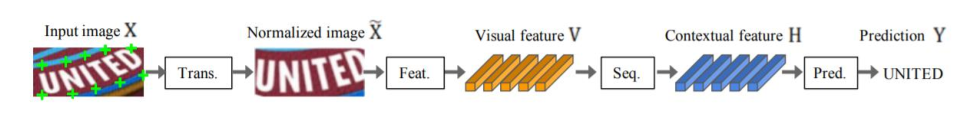
\includegraphics[width=5.5in,scale=1.8]{images/textrec.eps}
\caption[Text recognition framework]{Text recognition framework. Source: \citep{baek2019wrong}}
\label{fig:frame}
\end{figure}

An integrated framework that consists of four stages is proposed for scene text recognition as shown in Figure \ref{fig:frame}. It is as follows:
\begin{enumerate}
\item \textbf{Transformation:}
	The input image in natural scenes comes in arbitrary shapes like curved, vertical, irregular and diverse shapes. Thus the transformation stage uses the \gls{tps}, a variant of \gls{stn} to normalize the input image and transform it into a predefined rectangle.
\item \textbf{Feature extraction:}
	The feature extraction uses CNNs to estimate each character in the receptive field. Their framework has the option to select between ResNet, VGG, and RCNN architecture for feature extraction. We have used ResNet for feature extraction in our OCR engine.
\item \textbf{Sequence modelling:}
	Sequence modelling is used to model the contextual information within the sequence of characters using Bidirectional LSTM (BiLSTM) for robust predictions. 
\item \textbf{Prediction:}
	Attention (Attn) or \gls{ctc} is used to predict a sequence of characters for an input image. We have used Attn as a prediction module for our pre-trained model in this thesis. In the case of CTC, it enables the prediction of a non-fixed number of sequences despite the fixed number of features. The core of CTC seems to be that words can be combined by recognizing letters in each input column and removing repeated letters or blanks. On the other hand, Attn is said to automatically capture the flow of information in the input sequence to predict the output sequence. So, Attn helps the model learn a character-level language modelling that represents class dependencies in the output.
\end{enumerate}

\section{Google Vision OCR}
Google provides an \gls{api} that allows users to integrate many computer vision cloud services such as face detection, logo detection, object detection, text detection, etc to their framework \citep{googleapi}. One such commercial service is the cloud-based OCR that can recognize image files in multiple formats and convert them to text. The API must be enabled first to access the OCR engine and a key for the API needs to be generated. Then the text can be extracted from any number of images that are uploaded. In the work of \citep{compocrs}, they compared different OCR tools available in the market and showed that Google Vision OCR is one of the best tools for optical recognition. We have conducted experiments with the google vision OCR in addition to the proposed OCR to compare and evaluate how good is the proposed OCR engine.


\section{The overall framework}

The proposed framework includes the best generator model from the above-discussed GANs to preprocess the weathered steel type plates. Then the
generated image is passed into OCR engine to extract the text out of it.
\begin{figure}[H]
\centering
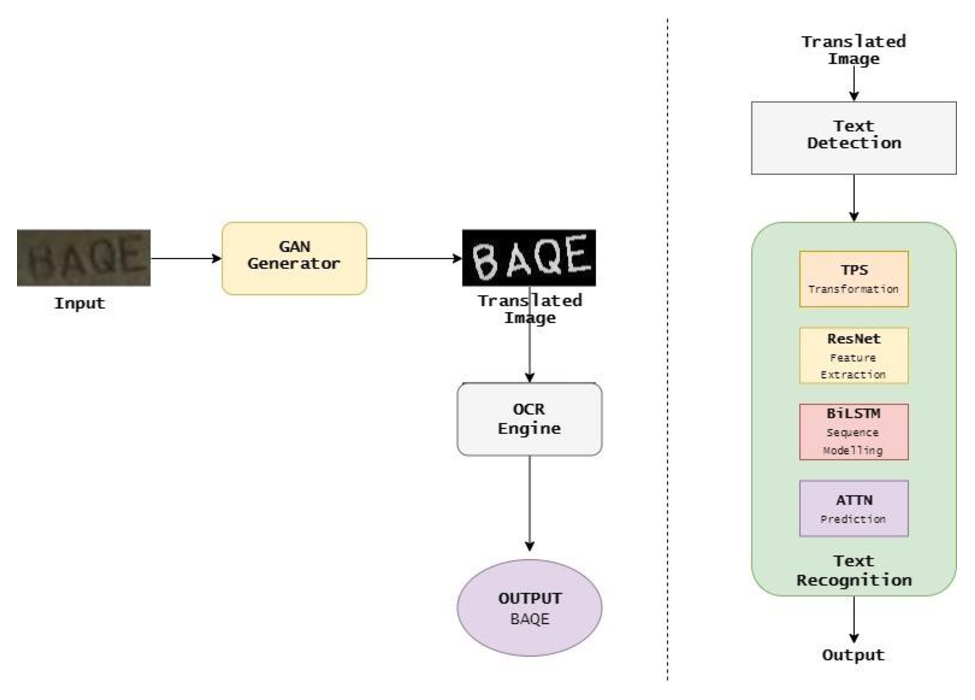
\includegraphics[width=5in]{images/overall.eps}
\caption{(a) The overall framework     (b) The proposed OCR }
\label{fig:framework}
\end{figure}
	
	In this thesis, we have studied two different OCR engines 1) Google Vision OCR and 2) The proposed CRAFT based OCR engine with integrated text detection and recognition models. The overall framework is shown in the left of Figure \ref{fig:framework}. 
\newline

	 The proposed OCR engine is shown in the right of Figure
\ref{fig:framework}. It consists of the CRAFT text detection model followed by the text recognition model. The text recognition model uses \gls{tps} for transformation, ResNet as feature extractor, BiLSTM for sequence modelling and Attn for prediction. 


	
\newpage
\chapter{Experiment}\label{ch:exp}
	This chapter describes in detail the implementation and experimental setup of the overall framework used in this thesis. In addition, Section \ref{sec:dataset} discusses in depth about the dataset of steel type plate images, the process of creating image pairs and synthetic data elaborately. Finally, Section \ref{sec:eval} describes the evaluation metrics used to measure the performances of all the GANs and OCR engines under study.

\section{Implementation}\label{sec:imp}
In this section, we list out the best hyperparameters for each method from the different settings that were tried out and their implementation in detail. For all the three GANs that were studied, we used the ADAM optimizer with the same values $\beta_1$ 0.5 and $\beta_2$ 0.999 for both generator and discriminator. We have used the PatchGAN discriminator for both pix2pix and CycleGAN experiments. We have performed experiments with different combinations for hyperparameters such as\\
i) Normalization \\
ii) Regularization using dropout \\
iii) Batch size with respect to multiple GPUs \\
iv) Size of the input image\\
v) Data augmentation using flip\\
vi) Learning rate\\
vii) Use of synthetic data\\
viii) Architecture for generator and discriminator\\

	The random search with qualitative evaluation was used for hyperparameter optimization. Many hyperparameters such as batch size, epoch, etc had little impact on the results of the training. For all the three GANs, the combination of parameters used in the original paper produced the best results. These settings are listed in the following table:

\begin{table}[H]
\resizebox{\textwidth}{!}{%
\begin{tabular}{@{}|c|c|c|c|@{}}
\toprule
                       & \textbf{Pix2pix}    & \textbf{CycleGAN}   & \textbf{FactorGAN}          \\ \midrule
\textbf{Batch Size}    & 4      & 2        & 25       \\ \midrule
\textbf{Learning Rate} & 0.002  & 0.002    & 0.001    \\ \midrule
\textbf{Optimizer}     & Adam   & Adam     & Adam     \\ \midrule
\textbf{beta1}         & 0.5    & 0.5      & 0.5      \\ \midrule
\textbf{beta2}         & 0.999  & 0.999    & 0.999    \\ \midrule
\textbf{Epoch}         & 200    & 200      & 200      \\ \midrule
\textbf{Dropout}       & No     & Yes      & No       \\ \midrule
\textbf{Normalization} & Batch  & Instance & Spectral \\ \midrule
\textbf{Generator}     & ResNet & ResNet   & U-Net     \\ \midrule
\textbf{Discriminator} & Patch discriminator & Patch discriminator & Convolutional discriminator \\ \bottomrule
\end{tabular}%
}
\caption{Best parameter setting used in the experiments for each GAN}
\label{tab:tabparam}
\end{table}

The original PyTorch implementation of GAN and OCR models that have been used for training can be found in the following repositories :
\newline
\begin{enumerate}
\item \textbf{Pix2pix \& CycleGAN} - \url{https://github.com/junyanz/pytorch-CycleGAN-and-pix2pix}

\item \textbf{FactorGAN} - \url{https://github.com/f90/FactorGAN}

\item \textbf{Text detection} - \url{https://github.com/clovaai/CRAFT-pytorch}

\item \textbf{Text detection pretrained model (craft-mlt-25k.pth)} - \url{https://drive.google.com/file/d/1Jk4eGD7crsqCCg9C9VjCLkMN3ze8kutZ/view}

\item \textbf{Text recognition} - \url{https://github.com/clovaai/deep-text-recognition-benchmark}

\item \textbf{TPS-ResNet-BiLSTM-Attn.pth} - The pretrained model for text recognition can be found in \url{https://drive.google.com/drive/folders/15WPsuPJDCzhp2SvYZLRj8mAlT3zmoAMW}
\end{enumerate}

	All the codes used in the thesis, latex files and the codes that are referenced from public repositories along with its respective licenses are included in the university GitLab repository. It can be cloned using the following URL: \url{https://www.uni-hildesheim.de/gitlab/panneers/thesis_steel_type_plate_recognition.git}.

\section{Experimental setup}
For our experiments, all codes are written in python and implemented in PyTorch. We have used other python libraries such as Numpy, Scipy, Pillow, Scikit-Learn. For training, we have used machines with a configuration having AMD Ryzen TR 2920X processor with 64 cores, 2 x 8 GB RTX 2070 Super X GPU, 128 GB RAM.

\section{Dataset}\label{sec:dataset}

This section provides a brief description of the dataset used in this thesis. Generally, the datasets for everyday objects are widely available. But for specific industrial use cases like in our case, it remains scarce. So, the data needs to be created from scratch.

\subsection{Data collection}
	Here, we introduce our strategies to dataset collection and processing. The following steps were performed to create the dataset:
\begin{enumerate}
\item A python script is written such that it crawls the steel type plate images from the google image search to create the dataset. 
\item Then the resulting images of web scraping were manually refined to remove the unnecessary images from the dataset. 
\item The images were cropped to remove the background information and to keep only the steel type plates part in the image.
\item In the middle of the experiment, few duplicate images were found in the dataset. Then these duplicate images were removed using a python script.
\item All the images in the dataset were resized to a uniform resolution of 600 x 400.
\item The final dataset consists of train, test and validation split with 366 in the train set, 30 in the validation set and 100 images for the testing set.
\end{enumerate}

\subsection{Label creation}
Since we use the image-to-image translation GAN models, the target labels corresponding to each input image needed to be created for training. The labels for every image is created in the following manner :

\begin{itemize}

\item Initially the RGB images in the dataset are converted to grayscale images.

\begin{figure}[H]
\centering
\begin{subfigure}{.47\textwidth}
  \centering
  \includegraphics[width=.7\linewidth]{images/L1.jpg}
  \caption{RGB image}
\end{subfigure}%
{\LARGE$\xrightarrow{}$}%
\begin{subfigure}{.47\textwidth}
  \centering
  \includegraphics[width=.7\linewidth]{images/L2.jpg}
  \caption{Grayscale image}
\end{subfigure}
\caption{RGB to Grayscale conversion}
\end{figure}

\item Then, we used the \textit{Photo Sketch} app in the iPad and highlighted the text part on top of each grayscale image manually using Apple pencil as shown in Figure \ref{fig:ann}. 

\begin{figure}[H]
\centering
\includegraphics[width=3in]{images/L3.jpg}
\caption{Annotated image}
\label{fig:ann}
\end{figure}

\item Now, the difference is calculated between the annotated image and the grayscale image using \textit{ImageOps} function from the Pillow library. The resulting image is shown in Figure \ref{fig:diff}.

\begin{figure}[H]
\centering
\begin{subfigure}{.49\textwidth}
  \centering
  \includegraphics[width=.9\linewidth]{images/L4.jpg}
  \caption{Difference image}
  \label{fig:diff}
\end{subfigure}%
\begin{subfigure}{.49\textwidth}
  \centering
  \includegraphics[width=.9\linewidth]{images/L5.jpg}
  \caption{Binary image}
  \label{fig:thres}
\end{subfigure}
\caption{The resulting image with better constrast between text and background}
\end{figure}

\item Finally the binary image is produced using an \textit{Adaptive Thresholding} function from the python OpenCV library. But thresholding step is skipped during training since it seemed to produce more noise in the translation results.

\begin{figure}[H]
\centering
\includegraphics[width=5in]{images/imagepair.jpg}
\caption{A steel type plate image with its input and output pair}
\label{fig:imgpair}
\end{figure}
\end{itemize}

	The final image pair sample used for training is shown in Figure \ref{fig:imgpair}.
\subsection{Synthetic dataset}
A framework to create a synthetic dataset is introduced in this thesis to generate images close to real steel type plates. The synthetic data supplement the original dataset since it has less than 400 image pairs and helps in reducing the manual effort of annotating more images.
\newline
\begin{wrapfigure}{r}{0.5\textwidth}
\centering
\includegraphics[width=0.4\textwidth]{images/template.jpg}
\caption{A sample template image}
\label{fig:template}
\end{wrapfigure}

	The Figure \ref{fig:template} shows a steel type plate template. More such templates are available for selection in the framework. The dictionary pool consists of around 750 image patches that contain different shapes of alphanumeric characters as well as word patches randomly cropped from the original images of steel type plates with its corresponding labels. Figure \ref{fig:syndata} shows some of the samples of cropped image patches present in the dictionary with its output pair.
\begin{figure}[H]
\centering
\includegraphics[width=5in]{images/syndata.jpg}
\caption{Sample image pairs in the dictionary pool}
\label{fig:syndata}
\end{figure}

The framework is built using python script and OpenCV libraries. At first, it randomly chooses a template of the steel plate. Once the template is selected, the framework loads the objects of the selected template class. 
\newline
\begin{figure}[H]
\centering
\includegraphics[width=5in]{images/synda1.jpg}
\caption{A synthetic image with its input and output pair}
\label{fig:syn}
\end{figure}

	It contains information such as the location of the templates, number of cropped areas and corresponding bounding box coordinates. Then, the framework picks a random item from the dictionary and fits these into each white boxes of the template. The generated synthetic image is shown in Figure \ref{fig:syn}. The framework has the option to vary the illumination and brightness of the generated image. Furthermore, it also has the functionality to add noises like gaussian, speckle, salt \& pepper, etc. 

\section{Evaluation metrics}\label{sec:eval}
The evaluation of the generative models is still an open research problem \citep{salimans2016improved}. The GAN generates realistically synthetic images and is often difficult to compare the performance of different GAN models with one another. \cite{borji2019pros} in their work, conducted a detailed study on the evaluation of GAN. According to their research, several methods have been introduced to evaluate GAN  yet there is no clear winner on which method captures the strengths and limitations of the model.
	The evaluation methods for GAN can be generally classified into two types: i) Quantitative evaluation and ii) Qualitative  evaluation

\subsection{Quantitative evaluation}
\cite{yang2018mri} used metrics such as \gls{mae}, \gls{psnr} to evaluate their work of image-to-image translation model. Similarly in this thesis, we have used MSE, SSIM and FID score to quantitatively measure the performance of the different GAN models. The synthetic images can be quantitatively evaluated with metrics such as MSE that calculate per-pixel-errors. This method calculates the average pixel difference between the ground truth images and the generated images. The MSE is not a great measure for performance indicators since it does not reveal anything about the quality or structural similarity of the image. Yet, higher MSE means the generated image is very different from the ground truth image. The MSE of two images x and y is given by

\begin{equation*}
MSE(x,y) = \frac{1}{m*n}\sum_{i=0}^{m-1}\sum_{j=0}^{n-1}[x(m,n) - y(m,n)]^2
\end{equation*}

SSIM proposed by \cite{wang2004image} can be used to measure the similarity and quality of generated images with respect to the ground truth. It compares the pixels of two images using three quantities such as luminance (I), contrast (C) and structure (S). For images x and y , it is given by,

\begin{align*}
I(x,y) = \dfrac{2\mu_x\mu_y + C_1}{\mu^2_x + \mu^2_y + C_1} \;\;\;
C(x,y) = \dfrac{2\sigma_x\sigma_y + C_2}{\sigma^2_x + \sigma^2_y + C_2} \;\;\;
S(x,y) = \dfrac{\sigma_{xy} + C_3}{\sigma_x \sigma_y + C_3}
\end{align*}

	where, $\mu_x,\mu_y,\sigma_x \; and \; \sigma_y$ denote the mean and standard deviation of pixel intensities between two images. $C_1, C_2 \; and \; C_3$ are constants added for numerical stability. The final SSIM score \citep{wang2004image} is given by
	
\begin{equation*}
SSIM(x,y) = I(x,y)^\alpha C(x,y)^\beta S(x,y)^\gamma
\end{equation*}

	where $\alpha, \beta \; and \; \gamma$ are the parameters to adjust the relative importance of I, C and S. The score ranges between 0 (Low similarity) and 1 (High similarity).

\subsection*{Frechet Inception Distance (FID)}
	The most commonly used method to evaluate the quality of generated images is to use classifiers pre-trained on real image distribution. Inception score is a measure that classifies if the synthetic images are realistic with the help of a classification network trained on real images. \citeauthor{heusel2017gans} proposed FID which is an improvised version of the Inception score. FID compares the Gaussian distribution of ground truth with generated images to quantify its quality. The FID score between real and generated images \citep{heusel2017gans} is given by 

\begin{equation*}
FID(r,g) = \lVert{\mu_r - \mu_g}\lVert_2^2 \; +  \; T_r(\Sigma_r + \Sigma_g - 2(\Sigma_r\Sigma_g)^{\frac{1}{2}})
\end{equation*}
	
It is shown that the FID score is more reliable, consistent and robust than the Inception score. Lower the FID score, better the quality of generated images.

\subsection{Qualitative evaluation}
The manual image inspection is a good starting point for qualitative analysis although visual comparison of real and generated images is difficult when the changes are very small.
The qualitative evaluation is not sufficient to determine the performance of the GAN. Therefore it is used together with the other metrics to evaluate the synthetic images such that it complements the quantitative evaluation. In this thesis, the synthetic image generated by three different GANs under study is visually distinguishable.
\subsection{Evaluation of OCR}
	For evaluating the OCR engines, we have conducted experiments with the test images before translation as well as the corresponding GAN translated images. These images are passed separately to both the proposed OCR engine and the commercial OCR tool like Google Vision. Finally, we have two outcomes for each OCR engine: i) character recognition of images without GAN translation and ii) character recognition of images using GAN translation. Then the output is compared with the annotations and the results are tabulated. We take into measures like the number of characters present in the text, the number of characters identified and the recognition rate in the name of OCR score. The OCR score is given by the number of characters identified correctly divided by the total number of texts present in the image. 
The following formula is used to calculate the OCR score: 
\begin{align*}
OCR \; score = \dfrac{Total \; number \; of \; characters \; identified \; correctly}{Total \; number \; of \; characters} * 100
\end{align*}

\newpage
\chapter{Results \& Discussion}\label{ch:results}
The results and discussion for all tests regarding both the GAN and OCR are presented in this chapter. Both the qualitative and quantitative results are provided for the evaluation of GAN models as discussed in the previous chapter. The quantitative results of GAN are discussed using the bar plots with metrics such as SSIM, FID and MSE while the qualitative results are discussed using visual results of test images from the output of the GAN generator. Then character recognition is evaluated using both the google vision API and the proposed integrated OCR engine. This chapter is concluded with the discussion of the effectiveness of GAN in terms of improvement in the character detection and recognition of the steel type plate images.

\section{Results of GAN}
Both the quantitative and qualitative results regarding the steel type plate images translated by the GAN models are presented below.

\subsection{Quantitative results}
As discussed earlier in the previous chapter, the GAN models are evaluated using three different metrics: i) FID, ii) SSIM and iii) MSE. The bar chart (Figure \ref{fig:fid}) below gives information about how the test images are evaluated using the FID metric. Lower FID indicates the better quality of generated images. The results obtained from the FID evaluation showed that the pix2pix model does well among the other models. The results of pix2pix have the lowest FID score of 15.09  and outperform other models by a significant margin. The use of synthetic data produces similar kinds of results for the pix2pix model. The CycleGAN performs the worst with a score of 51.76. This can be explained by the fact that the model is trained in an unsupervised manner with fewer data points. The FactorGAN produced slightly better results compared to the CycleGAN with a score of 32.35, but not as good as pix2pix.

\begin{figure}[H]
\centering
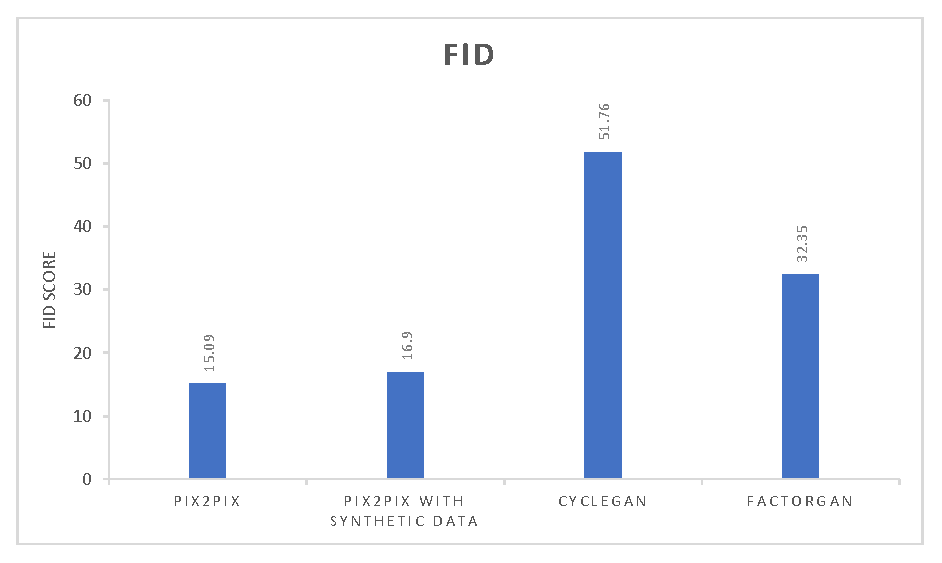
\includegraphics[width=4in]{images/FID.eps}
\caption{Experimental results for FID}
\label{fig:fid}
\end{figure}


In a search for a still more accurate result, the pix2pix model is trained with the synthetic dataset along with the real dataset. This also produced similar results as that of the pix2pix model trained only with the original image dataset. The difference between both the results were very minute as seen in the quantitative results and could not be differentiated during the qualitative evaluation. The CycleGAN and FactorGAN architecture have 4 networks each in total as discussed in Chapter \ref{ch:method}. The time taken for training both the models is very high in general. Also, they produced the worst results compared to the pix2pix while using the original dataset. Therefore the experiments with the synthetic dataset were not conducted for both CycleGAN and FactorGAN.  
\newline
	
	The SSIM score gives the similarity between ground truth data and the output of the generator for the test images. Higher SSIM indicates better quality of generated images. The chart shown in the Figure \ref{fig:ssim} shows the SSIM scores evaluated for different GAN models. The results of SSIM is exactly similar to the FID evaluation. The model that has the best SSIM score is pix2pix with a similarity score of 0.8. The model trained with synthetic dataset + pix2pix produces similar results that of pix2pix with a score of 0.79. The SSIM score for FactorGAN and CycleGAN is very low compared to other models with a score of 0.74 and 0.69 respectively.

\begin{figure}[H]
\centering
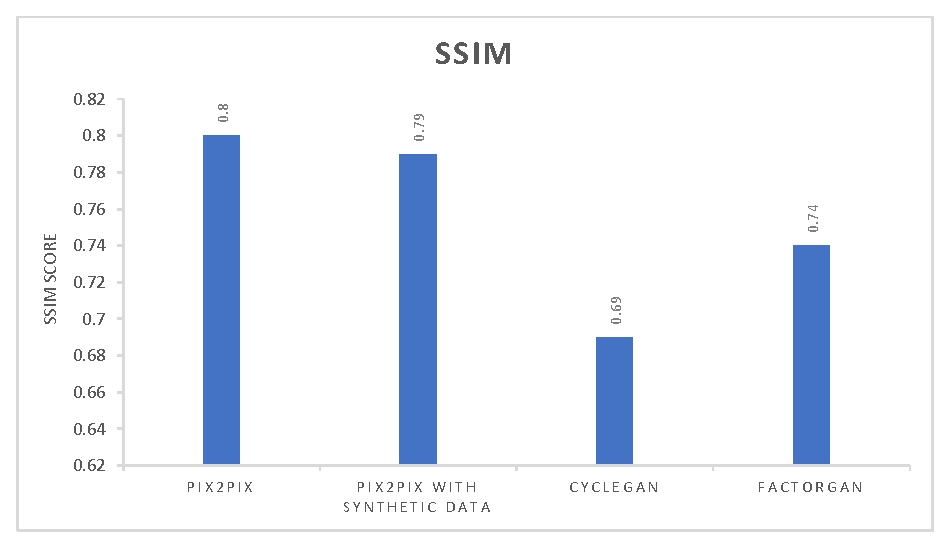
\includegraphics[width=4in]{images/ssim.eps}
\caption{Experimental results for SSIM}
\label{fig:ssim}
\end{figure}

	The MSE is calculated by squaring the absolute difference between the pixels of ground truth and the generated image. The result of this experiment is shown in Figure \ref{fig:mse}. It is seen that the model trained with synthetic data with pix2pix GAN has the least error whereas the CycleGAN model with a MSE of 5739.08 performs the worst. The MSE for pix2pix does not differ much from the best model with the value of 3377.56 while the MSE of FactorGAN is 3664.83.

\begin{figure}[H]
\centering
\includegraphics[width=4in]{images/mse.eps}
\caption{Experimental results for MSE}
\label{fig:mse}
\end{figure}

\subsection{Qualitative results}
The qualitative results are evaluated by manual visual inspection of translated test images for all three different GANs. Figures \ref{test1} - \ref{test3} show how different models perform when translating the image from unclear to a clearer image. Since it is not possible to display all the images, we have shown the test results of three sample images with their ground truth and corresponding translation by three different GANs. 
\newline	

	
	Both the quantitative and qualitative results of the experiment can be found in the GitLab link shared in Section \ref{sec:imp}.  It can also be accessed using the shared google drive \url{https://drive.google.com/drive/folders/1lMbM0bjMx1LoIyi8cyV7Nz1Gy5yUisXB?usp=sharing}. The qualitative results support the findings of the quantitative results. From the results, it can be seen that the pix2pix model successfully generate images very close to ground truth images. The use of ResNet as a feature extractor combined with paired dataset and techniques such as random cropping of the input image to the size of 256 x 256 for each epoch during training contributed to the success of the pix2pix model. This complements the experiments for quantitative evaluation. The misclassified characters for pix2pix are mostly repetitive. In rare cases, the texts were incorrectly transformed or missed. For example, the characters such as 'D', '/', 'G' in the steel plates are misclassified as '0', '7', '6' respectively.
\newline	
	
		
\begin{figure}[H]
\begin{tabular}{cc}
\includegraphics[width=65mm]{images/i2.jpg} &   \includegraphics[width=65mm]{images/g2.jpg} \\
(a) Input & (b) Ground Truth \\[6pt]
 \includegraphics[width=65mm]{images/p2.jpg} &   \includegraphics[width=65mm]{images/c2.jpg} \\
(c) Pix2pix & (d) CycleGAN \\[6pt]
\multicolumn{2}{c}{\includegraphics[width=65mm]{images/f2.jpg} }\\
\multicolumn{2}{c}{(e) FactorGAN}
\end{tabular}
\caption{Test result: Sample 1}
\label{test1}
\end{figure}

The CycleGAN produces the worst results though it uses ResNet as a feature extractor. From Figures \ref{test1} - \ref{test3}, it can be seen that CycleGAN misses a lot of text areas compared to the annotated images. It gives decent output only when the text area is clear in the original image. It fails to segment the characters when the corresponding area in the input image has even a little bit of noise such as reflection or under different lighting conditions.  Thus CycleGAN skips a lot of characters and could not translate the complete structure of the input image. Thus it results in huge MSE loss, worst SSIM
\begin{figure}[H]
\begin{tabular}{cc}
\includegraphics[width=65mm]{images/i1.jpg} &   \includegraphics[width=65mm]{images/g1.jpg} \\
(a) Input & (b) Ground Truth \\[6pt]
 \includegraphics[width=65mm]{images/p1.jpg} &   \includegraphics[width=65mm]{images/c1.jpg} \\
(c) Pix2pix & (d) CycleGAN \\[6pt]
\multicolumn{2}{c}{\includegraphics[width=65mm]{images/f1.jpg} }\\
\multicolumn{2}{c}{(e) FactorGAN}
\end{tabular}
\caption{Test result: Sample 2}
\label{test2}
\end{figure}
\noindent
and FID score as found during the quantitative evaluation. The use of unsupervised learning, unpaired dataset and insufficient data points are the probable reasons for the failure of CycleGAN.
\newline	

	
\begin{figure}[H]
\begin{tabular}{cc}
\includegraphics[width=65mm]{images/i4.jpg} &   \includegraphics[width=65mm]{images/g4.jpg} \\
(a) Input & (b) Ground Truth \\[6pt]
 \includegraphics[width=65mm]{images/p4.jpg} &   \includegraphics[width=65mm]{images/c4.jpg} \\
(c) Pix2pix & (d) CycleGAN \\[6pt]
\multicolumn{2}{c}{\includegraphics[width=65mm]{images/f4.jpg} }\\
\multicolumn{2}{c}{(e) FactorGAN}
\end{tabular}
\caption{Test result: Sample 3}
\label{test3}
\end{figure}

The much expected FactorGAN did not live up to its expectations either. Even though \citeauthor{stoller2019training}'s hypothesis of improved segmentation accuracy over CycleGAN still holds true for our experiments with steel type plates dataset, the pix2pix GAN produces results which are far better from the results of FactorGAN. This may be because our dataset is very different from the cityscapes dataset \citep{cordts2016cityscapes} that was used in the \citeauthor{stoller2019training} experiments for training FactorGAN. The classes of cityscapes dataset fall under seven groups like human, vehicle, construction, etc,. Their classes have a broader boundary and include large objects whereas our steel type plate dataset mainly consists of two classes: characters and background which have a finer class boundary. The results of FactorGAN show that it captures all the necessary character segmentation areas like pix2pix but the translations are very blurry and cannot be used for character recognition. Thus the FactorGAN has only the second-best results during the quantitative evaluation. 
\newline

	In general, the translation becomes problematic when the font size of the text present in the images is very small or very big. Also, it was noted in the results that embossed texts were not correctly transformed in many test cases. This can be due to the fact that the images in our dataset had more samples of engraved texts than embossed texts. 
\newline
	
	From both the quantitative and qualitative evaluation, the pix2pix model stands out as the best model. So the final proposed framework consists of a pix2pix model for translating the noisy steel plates to clear images. 
	
\section{Results of OCR}
For evaluating the efficiency of the use of GAN for character recognition, we randomly cropped the 30 test images to the size 256 x 256 and translated it using pix2pix GAN. Both the original image and its GAN translated image is passed into the OCR engine for character recognition. In this thesis we experimented with two different OCR engines: i) The commercial OCR engine using Google Vision API ii) The proposed CRAFT based OCR engine. The results of the experiments are tabulated in Tables \ref{tab:ocrtab1} - \ref{tab:ocrtab3}.				

\subsection{Evaluation using Google Vision OCR}
	Table \ref{tab:ocrtab1} compares the character recognition before and after the use of the GAN translated image using Google Vision OCR. The table presents the total number of characters present in the test images, the number of characters recognized by the Google Vision OCR engine and the average OCR Score. The number of characters recognized is further split into characters correctly identified, incorrectly identified and missed.

\begin{table}[H]
\resizebox{\textwidth}{!}{%
\begin{tabular}{@{}|c|c|c|c|c|c|c|@{}}
\toprule
 &
  \textbf{\begin{tabular}[c]{@{}c@{}}Total number of \\ characters\end{tabular}} &
  \textbf{\begin{tabular}[c]{@{}c@{}}Characters \\ recognized\end{tabular}} &
  \textbf{\begin{tabular}[c]{@{}c@{}}Correctly \\ identified\end{tabular}} &
  \textbf{\begin{tabular}[c]{@{}c@{}}Incorrectly \\ identified\end{tabular}} &
  \textbf{\begin{tabular}[c]{@{}c@{}}Characters \\ missed\end{tabular}} &
  \textbf{OCR Score} \\ \midrule
\textbf{\begin{tabular}[c]{@{}c@{}}Character recognition\\  without GAN\end{tabular}} &
  1303 &
  1054 &
  914 &
  140 &
  249 &
  67.06 \\ \midrule
\textbf{\begin{tabular}[c]{@{}c@{}}Character recognition \\ with GAN\end{tabular}} &
  1303 &
  1287 &
  1104 &
  183 &
  16 &
  84.09 \\ \bottomrule
\end{tabular}%
}
\caption{Character recognition with and without GAN using Google Vision OCR engine}
\label{tab:ocrtab1}
\end{table}

\begin{figure}[H]
\centering
\includegraphics[width=5in]{images/ocrcomp3.eps}
\caption{Evaluation of character recognition using Google Vision}
\label{fig:ocrcomp3}
\end{figure}

 The total number of characters present in the test images is 1303. The total number of characters recognized for original images is 1054 whereas the total number of characters recognized significantly increased to 1287 when using their corresponding GAN translated images. Also, the characters missed are drastically reduced from 249 to 16 when using GAN translated images. The results in the above table are plotted using a bar chart in Figure \ref{fig:ocrcomp3}.



\subsection{Evaluation using the proposed OCR}


The same experiment is repeated for the proposed OCR engine with the same test images for evaluating the efficiency of the use of GAN in character recognition. The results are tabulated in Table \ref{tab:ocrtab2}. It compares the character recognition before and after the use of GAN translated image using the proposed OCR. Similar to Table \ref{tab:ocrtab1}, this table presents the total number of characters present in the test images, the number of characters recognized by the proposed OCR engine and its average OCR score.
\begin{table}[H]
\resizebox{\textwidth}{!}{%
\begin{tabular}{@{}|c|c|c|c|c|c|c|@{}}
\toprule
 &
  \textbf{\begin{tabular}[c]{@{}c@{}}Total number of \\ characters\end{tabular}} &
  \textbf{\begin{tabular}[c]{@{}c@{}}Characters \\ recognized\end{tabular}} &
  \textbf{\begin{tabular}[c]{@{}c@{}}Correctly \\ identified\end{tabular}} &
  \textbf{\begin{tabular}[c]{@{}c@{}}Incorrectly \\ identified\end{tabular}} &
  \textbf{\begin{tabular}[c]{@{}c@{}}Characters\\  missed\end{tabular}} &
  \textbf{OCR score} \\ \midrule
\textbf{\begin{tabular}[c]{@{}c@{}}Character recognition \\ without GAN\end{tabular}} &
  1303 &
  1036 &
  830 &
  206 &
  267 &
  61.78 \\ \midrule
\textbf{\begin{tabular}[c]{@{}c@{}}Character recognition\\  with GAN\end{tabular}} &
  1303 &
  1267 &
  1094 &
  173 &
  36 &
  84.37 \\ \bottomrule
\end{tabular}%
}
\caption{Character recognition with and without GAN using the proposed OCR engine}
\label{tab:ocrtab2}
\end{table}

In case of proposed OCR, the character recognition is increased from 1036 to 1267 when using GAN translated images. Also, the characters missed are reduced from 267 to 36 when using GAN translated images. The results in the above table are plotted using a bar chart in Figure \ref{fig:ocrcomp3}.

	
\begin{figure}[H]
\centering
\includegraphics[width=5in]{images/ocrcomp4.eps}
\caption{Evaluation of character recognition using the proposed OCR engine}
\label{fig:ocrcomp4}
\end{figure}

Tables \ref{tab:ocrtab1} and \ref{tab:ocrtab2} show that the average OCR score for Google Vision OCR is increased from 67.06 \% to 84.09 \% while the average OCR score is massively increased from 61.78 \% to 84.37 \% when using the GAN translated image.

\subsection{Comparison of OCR engines}
This section compares the impact of image-to-image translation GAN on both the OCR engine in terms of improvement of character recognition. Table \ref{tab:ocrtab3} presents the comparison of both the OCR engines in terms of improvement in character recognition when using GAN. 
\newline

	As discussed above in the tables \ref{tab:ocrtab1} \& \ref{tab:ocrtab2}, when using GAN translated image, the character recognition i.e. the detection of the number of characters in the steel type plates is improved by 20.09 \% for the proposed OCR. Even for the commercial OCR tool like Google Vision, the character recognition of steel type plates is improved by 20.16 \%. 
\begin{table}[H]
\resizebox{\textwidth}{!}{%
\begin{tabular}{@{}|c|c|c|@{}}
\toprule
\textbf{OCR engine} &
  \textbf{\begin{tabular}[c]{@{}c@{}}Improvement of character \\ recognition using GAN \\ translated Image\end{tabular}} &
  \textbf{\begin{tabular}[c]{@{}c@{}}Percentage increase\\  in OCR Score\end{tabular}} \\ \midrule
\textbf{The proposed OCR} &
  20.09 &
  36.57 \\ \midrule
\textbf{Google Vision} &
  20.16 &
  25.39 \\ \bottomrule
\end{tabular}%
}
\caption{Comparison of impact of GAN on both OCR engines}
\label{tab:ocrtab3}
\end{table}

Similarly, the OCR score for Google Vision is improved by 25.39 \% while for the proposed OCR, it has been massively increased by 36.57 \%. This is graphically represented using a bar chart in Figure \ref{fig:ocrcomp5}.


\begin{figure}[H]
\centering
\includegraphics[width=5in]{images/ocrcomp5.eps}
\caption{Comparison of impact of GAN on both OCR engines}
\label{fig:ocrcomp5}
\end{figure}
\newpage
\chapter{Conclusion}\label{ch:conclusion}
This chapter concludes the thesis with the contributions of the work with final comments on the results from the previous chapter. Also, we have addressed the limitations and the scope for future work.

\section{Summary}
The goal of the thesis is to investigate the use of the image-to-image translation GANs in improving the character recognition accuracy of steel type plate images. A framework has been introduced in this thesis to create a synthetic dataset of steel type plates along with its label pair to supplement the original dataset. We have studied three different image-to-image translation GAN approaches for translating the images of unclear steel type plates into clear images. These GAN models are evaluated both using the quantitative and qualitative metrics. After evaluation, it is found that the pix2pix generator works best. Thus the overall framework consists of pix2pix generator integrated with the OCR engine. The following are the answers to the research questions stated in this thesis:

\begin{enumerate}
\item \textit{Can an image-to-image translation GAN be used to improve the accuracy of character recognition for the images of weathered steel type plates?}

Yes. From the experimental results of the thesis, it has been proved that image-to-image translation GAN models can be used for improving the accuracy of the OCR engines. For even the benchmark commercial OCR engine like Google Vision, our model has improved the character recognition of steel type plates by 25.39 \% measured in terms of OCR score. Similarly, for the proposed OCR engine, the score has been massively increased by almost 37 \% after using GAN.

\item \textit{Can the findings of \citeauthor{CycleGAN2017} and \citeauthor{stoller2019training} be used to make up for the few image pairs in the steel type plate dataset?}

No, the experimental results show that the techniques of \citeauthor{CycleGAN2017}'s unpaired dataset and \citeauthor{stoller2019training} training incomplete data points did not work well for our steel type plate dataset. Generally, the success of any deep neural networks depends heavily on the size of the dataset used for training. Our training dataset has a size of 366 image pairs. To tackle this problem of the dataset with fewer data points, various techniques such as data augmentation, random cropping of the input to a smaller size (256 x 256) than the load size (600 x 400) for each epoch during training are employed. Besides, a framework to generate a synthetic dataset has been introduced to supplement the original dataset. Even though the number of image pairs present in the training set was sufficient enough to train the image-to-image GAN models successfully, more image pairs can still produce a more robust generator model. Notably, the pix2pix model without any data augmentation techniques produced splendid results just with approximately 150 - 200 image pairs.

\item \textit{How to evaluate the three different image-to-image translation GAN models under the scope of the thesis and choose the optimal model for the proposed steel type plate recognition system?}

We have chosen the best GAN using both quantitative and qualitative evaluations. Metrics such as FID, SSIM and MSE are used for the quantitative measure while a manual inspection is used for qualitative measure. From the experimental results, the optimal GAN model was found out to be pix2pix.


\item \textit{How good is the proposed OCR engine compared to a commercial OCR engine like Google Vision? How can the performance of the overall framework be measured?}

We have compared the proposed OCR engine with one of the benchmark OCR engines like Google Vision. We have introduced a metric called OCR score for measuring the performance of the OCR engine. It is found that character recognition is improved by 20 \% for both OCR engines when using the translated images. Likewise, after using GAN, the OCR score for Google vision OCR has been increased from 67 \% to 84 \% and for the proposed OCR engine, it is increased from 62 \% to 84 \%.

\end{enumerate}

\section{Limitations}
The main limitation of training any image-to-image translation model is the availability of data pairs. In our thesis, we used a small dataset of less than 400 image pairs. The current practice of manually annotating the images and creating a label pair is more time consuming and costly. Even the framework for generating synthetic steel type plate images is limited to the dictionary pool of manually cropped patches. Also, manually generated labels lack uniformity and have a high human bias.   

\section{Future works}
	Till now, there has been only a little work done in using GANs for OCR. The use of GANs in OCR has great potential and has scope for several promising applications like our steel type plate recognition. As future work, the overall system can be modified such that the model learns the loss function based on the output of the OCR engine directly as a combined loss instead of training image-to-image translation and OCR engine separately.


%%%%%%%%%%%%%%%%%%%%%%%%%%%%%%%%%%%%%%%%%
\newpage
\pagenumbering{gobble}
%{\setstretch{1.0}
\begin{thebibliography}{25}


\bibitem{saraee_et_al}
M. Saraee, S. White \& J. Eccleston, “A data mining approach to analysis and prediction of movie ratings”, University of Salford, England, The Fifth International Conference on Data Mining, Text Mining and their Business Applications, 15-17 September 2004, pp 344- 352.

\bibitem{role_factors_prediction_movie}
Bhave, A., Kulkarni, H., Biramane, V., \& Kosamkar, P. (2015, January). Role of different factors in predicting movie success. In 2015 International Conference on Pervasive Computing (ICPC) (pp. 1-4). IEEE.
 
\bibitem{actors_factor}
Wallace, W. T., Seigerman, A., \& Holbrook, M. B. (1993). The role of actors and actresses in the success of films: How much is a movie star worth?. Journal of cultural economics, 1-27.

\bibitem{star_factor}
De Vany, A., \& Walls, W. D. (1999). Uncertainty in the movie industry: Does star power reduce the terror of the box office?. Journal of cultural economics, 23(4), 285-318.

\bibitem{movie_success_problem}
Sharda, R., \& Delen, D. (2006). Predicting box-office success of motion pictures with neural networks. Expert Systems with Applications, 30(2), 243-254.

\bibitem{movie_forecastin_dnn}
Ghiassi, M., Lio, D., \& Moon, B. (2015). Pre-production forecasting of movie revenues with a dynamic artificial neural network. Expert Systems with Applications, 42(6), 3176-3193.

\bibitem{movie_forecasting_bpnn}
Zhang,  L.,  Luo,  J.,  \&  Yang,  S.  (2009).  Forecasting  box  office  revenueof movies with BP neural network. Expert Systems with Applications,36(3), 6580-6587.

\bibitem{statista_movies_released}
Statistics of movies released since 2001, https://www.statista.com/statistics/187122/movie-releases-in-north-america-since-2001/, visited online on January 25th, 2020

\bibitem{ltc}
Varol, G., Laptev, I., \& Schmid, C. (2017). Long-term temporal convolutions for action recognition. IEEE transactions on pattern analysis and machine intelligence, 40(6), 1510-1517.
 
\bibitem{lstm}
Hochreiter, S., \& Schmidhuber, J. (1997). Long short-term memory. Neural computation, 9(8), 1735-1780.

\bibitem{resnet}
K. He, X. Zhang, S. Ren and J. Sun, "Deep Residual Learning for Image Recognition," 2016 IEEE Conference on Computer Vision and Pattern Recognition (CVPR), Las Vegas, NV, 2016, pp. 770-778.

\bibitem{imdb}
Internet Movie Database, https://www.imdb.com/interfaces/, accessed online March 17th

\bibitem{kim_et_al}
T. Kim, J. Hong, and P. Kang. (2015). Box office forecasting using machine learning algorithms based on SNS data.

\bibitem{travis_et_al}
Travis Ginmu Rhee and Farhana Zulkernine. 2016. Predicting movie box office profitability: a neural network approach. In 2016 15th IEEE International Conference on Machine Learning and Applications (ICMLA), pages 665–670. IEEE.

\bibitem{sameer_et_al}
Sameer Ranjan Jaiswal and Divyansh Sharma. 2017. Predicting success of bollywood movies using machine learning techniques. In Proceedings of the 10th Annual ACM India Compute Conference on ZZZ, pages 121–124. ACM.

\bibitem{chen_a}
A. Chen, “Forecasting gross revenues at the movie box office,” Working paper, University of Washington Seattle, WA, June 2002.
 
\bibitem{winners_and_loosers}
Simonoff, J. S., \& Sparrow, I. R. (2000). Predicting movie grosses: Winners and losers, blockbusters and sleepers. Chance, 13(3), 15-24.

\bibitem{shawney_et_al}
M. S. Sawhney and J. Eliashberg, “A parsimonious model for forecasting gross box-office revenues of motion
pictures,” Marketing Science, vol. Vol. 15, No. 2, pp.
113–131, 1996.

\bibitem{Sitaram_Asur}
Sitaram Asur and Bernardo A. Huberman, “Predicting the Future with Social Media,” http://arxiv.org/abs/1003.5699, March 2010.

\bibitem{reddy_et_al}
Reddy, A. S. S., Kasat, P., \& Jain, A. (2012). Box-office opening prediction of movies based on hype analysis through data mining. International Journal of Computer Applications, 56(1), 1-5.

\bibitem{Nahid_Quader}
Quader, N., Gani, M. O., \& Chaki, D. (2017, December). Performance evaluation of seven machine learning classification techniques for movie box office success prediction. In 2017 3rd International Conference on Electrical Information and Communication Technology (EICT) (pp. 1-6). IEEE.

\bibitem{apala_et_al}
Apala, K. R., Jose, M., Motnam, S., Chan, C. C., Liszka, K. J., \& de Gregorio, F. (2013, August). Prediction of movies box office performance using social media. In 2013 IEEE/ACM International Conference on Advances in Social Networks Analysis and Mining (ASONAM 2013) (pp. 1209-1214). IEEE.

\bibitem{Yao_zhou}
Zhou, Y., Zhang, L., \& Yi, Z. (2019). Predicting movie box-office revenues using deep neural networks. Neural Computing and Applications, 31(6), 1855-1865.

\bibitem{ozkan_et_al}
K. Ozkan, O. N. Atak, and S. Işik. "Using movie posters for prediction of box-office revenue with deep learning approach." 2018 26th Signal Processing and Communications Applications Conference (SIU). IEEE, 2018.

\bibitem{gevaria_et_al}
Gevaria, K., Wagh, R., \& D'mello, L.R. (2015). Movie Attendance Prediction.

\bibitem{mashall_et_all}
Marshall, P., Dockendorff, M., \& Ibanez, S. (2013). A forecasting system for movie attendance.

\bibitem{zhang_et_al}
Zhang, Xu., Hou, Guangming., Dong, Weijia., Modelling movie attendance with seasonality: evidence from China, Applied Economics Letters. Nov2017, Vol. 24 Issue 19, p1351-1357. 7p. 

\bibitem{merlin_20fox}
Hsieh, C., Campo, M., Taliyan, A., Nickens, M., Pandya, M., \& Espinoza, J.J. (2018). Convolutional Collaborative Filter Network for Video Based Recommendation Systems. ArXiv, abs/1810.08189.

\bibitem{campo_et_al}
Miguel Campo, Cheng-Kang Hsieh, Matt Nickens, J. J. Espinoza, Abhinav Taliyan, Julie Rieger, Jean Ho, Bettina Sherick:
Competitive Analysis System for Theatrical Movie Releases Based on Movie Trailer Deep Video Representation. CoRR abs/1807.04465 (2018)

\bibitem{Wang_et_al}
H. Wang, N. Wang, and D.-Y. Yeung. Collaborative
deep learning for recommender systems. In
Proceedings of the 21th ACM SIGKDD International
Conference on Knowledge Discovery and Data Mining,
pages 1235–1244. ACM, 2015

\bibitem{Li_et_al}
X. Li and J. She. Collaborative variational
autoencoder for recommender systems. In Proceedings
of the 23rd ACM SIGKDD International Conference
on Knowledge Discovery and Data Mining, pages
305–314. ACM, 2017

\bibitem{ilsvrc_15}
The ILSVRC 2015 ImageNet Competition, http://image-net.org/challenges/LSVRC/2015/, accessed online March 3rd, 2020

\bibitem{coco_19}
Coco competition, http://cocodataset.org/home, accessed online March 3rd, 2020

\bibitem{rnn}
Rumelhart, David E.; Hinton, Geoffrey E.; Williams, Ronald J. (1986-10-09). "Learning representations by back-propagating errors". Nature. 323 (6088): 533–536. doi:10.1038/323533a0. ISSN 1476-4687.

\bibitem{movie_trailer_types}
Finsterwalder, J., Kuppelwieser, V.G., de Villiers, M. (2012) The effects of film trailers on shaping consumer expectations in the entertainment industry—A qualitative analysis. Journal of Retailing and Consumer Services, 19(6), pp. 589-595.
 
\bibitem{kernel_dimension}
D. Tran, L. Bourdev, R. Fergus, L. Torresani, and M. Paluri, “Learning spatiotemporal features with 3D convolutional networks,” in ICCV, 2015.

\bibitem{adam_optimizer}
Adam: A Method for Stochastic Optimization
D. Kingma, and J. Ba.(2014) Published as a conference paper at the 3rd International Conference for Learning Representations, San Diego, 2015.

\bibitem{imagenet}
ImageNet dataset link, http://www.image-net.org/, visited on February 2nd, 2020 

\bibitem{chen_gross_revenues}
Chen, A. (2002). Forecasting gross revenues at the movie box office. University of Washington, Seattle.
 
\bibitem{lash_et_al}
Lash, M. T., \& Zhao, K. (2016). Early predictions of movie success: The who, what, and when of profitability. Journal of Management Information Systems, 33(3), 874-903.
  
\bibitem{Simonyan_et_al}
Simonyan, K., \& Zisserman, A. (2014). Two-stream convolutional networks for action recognition in videos. In Advances in neural information processing systems (pp. 568-576).


% \bibitem{Karpathy_et_al}
% Karpathy, A., Toderici, G., Shetty, S., Leung, T., Sukthankar, R., \& Fei-Fei, L. (2014). Large-scale video classification with convolutional neural networks. In Proceedings of the IEEE conference on Computer Vision and Pattern Recognition (pp. 1725-1732).
 
% \bibitem{wang_et_al}
% Wang, L., Xiong, Y., Wang, Z., \& Qiao, Y. (2015). Towards good practices for very deep two-stream convnets. arXiv preprint arXiv:1507.02159.


% \bibitem{Feichtenhofer_et_al}
% Feichtenhofer, C., Pinz, A., \& Zisserman, A. (2016). Convolutional two-stream network fusion for video action recognition. In Proceedings of the IEEE conference on computer vision and pattern recognition (pp. 1933-1941).
 
% \bibitem{tran_et_al}
% Tran, D., Bourdev, L., Fergus, R., Torresani, L., \& Paluri, M. (2015). Learning spatiotemporal features with 3d convolutional networks. In Proceedings of the IEEE international conference on computer vision (pp. 4489-4497).
 
\bibitem{ji_et_al}
Ji, S., Xu, W., Yang, M., \& Yu, K. (2012). 3D convolutional neural networks for human action recognition. IEEE transactions on pattern analysis and machine intelligence, 35(1), 221-231.
 
\bibitem{taylor_et_al}
Taylor, G. W., Fergus, R., LeCun, Y., \& Bregler, C. (2010, September). Convolutional learning of spatio-temporal features. In European conference on computer vision (pp. 140-153). Springer, Berlin, Heidelberg.

\end{thebibliography}
}
\bibliographystyle{apalike}
\bibliography{Bibliography} 
\end{document}